\documentclass[12pt]{article}

% ----------------------------
% Page / font / spacing
% ----------------------------
\usepackage[letterpaper,margin=1in]{geometry}
\usepackage[T1]{fontenc}
\usepackage{lmodern}    % clean, embedded fonts in PDF
\usepackage{microtype}  % better PDF typography

\usepackage{setspace}
\onehalfspacing         % SSRN용으로는 보통 1.5 권장 (원하시면 \doublespacing로 변경)
\usepackage{tikz}
\usetikzlibrary{positioning, arrows.meta, fit, backgrounds, calc}
% ----------------------------
% Math
% ----------------------------
\usepackage{amsmath,amssymb,amsfonts}
\usepackage{tikz}
\usepackage{pgfplots}
\usetikzlibrary{positioning, arrows.meta, fit, backgrounds, calc}

% ----------------------------
% Figures / tables
% ----------------------------
\usepackage{graphicx}
\usepackage{booktabs}
\usepackage{siunitx}
\usepackage{threeparttable}
\usepackage{multirow, makecell, pgfplots}
\pgfplotsset{compat=1.18}
\usepackage{adjustbox}
\usepackage{array}
\usepackage{caption}
\usepackage{subcaption}
\usepackage{pdflscape}

% Custom column types
\newcolumntype{L}[1]{>{\raggedright\arraybackslash}m{#1}}
\newcolumntype{C}[1]{>{\centering\arraybackslash}m{#1}}
\newcolumntype{R}[1]{>{\raggedleft\arraybackslash}m{#1}}

% ----------------------------
% Citations
% ----------------------------
\usepackage[round]{natbib}

% ----------------------------
% Authors / affiliations
% ----------------------------
\usepackage[affil-it]{authblk}

% ----------------------------
% Colors (optional; keep if you use \red / \blue)
% ----------------------------
\usepackage{xcolor}
\newcommand{\red}[1]{{\color{red}#1}}
\newcommand{\blue}[1]{{\color{blue}#1}}

% ----------------------------
% Theorems / proof
% ----------------------------
\newtheorem{theorem}{Theorem}
\newtheorem{corollary}[theorem]{Corollary}
\newtheorem{proposition}{Proposition}
\newtheorem{hyp}{Hypothesis}
\newtheorem{subhyp}{Hypothesis}[hyp]
\renewcommand{\thesubhyp}{\thehyp\alph{subhyp}}

\newenvironment{proof}[1][Proof]{\noindent\textbf{#1.} }{\ \rule{0.5em}{0.5em}}

% ----------------------------
% Footnotes as endnotes (SSRN에서는 보통 footnote 그대로를 권장)
% 원래처럼 endnotes를 쓰시려면 아래 2줄을 주석 해제하세요.
% ----------------------------
% \usepackage{endnotes}
% \let\footnote=\endnote

% ----------------------------
% Hyperref (load last)
% ----------------------------
\usepackage[hidelinks]{hyperref}
\hypersetup{
  pdftitle={Interpreting News for Volatility: An Attention-Weighted HAR Framework},
  pdfauthor={Bong-Gyu Jang and Younwoo Jeong},
  pdfkeywords={Realized Volatility; Volatility Forecasting; HAR; Textual Information; Attention; Interpretable Machine Learning},
  pdfcreator={LaTeX}
}
\begin{document}

% ----------------------------
% Title block (SSRN-friendly: title + abstract on page 1)
% ----------------------------
\title{How Long Does News Move Crypto? Learning Decay Signals for High-Frequency Volatility Forecasting}

\author[1]{Bong-Gyu Jang}
\author[1]{Younwoo Jeong\thanks{Corresponding author: \texttt{younwoo48@postech.ac.kr}.}}
\author[1]{Juhwan Park}
\affil[1]{Pohang University of Science and Technology}

% SSRN 제출 폼에서 “Date paper was written”은 필수 입력 항목이므로 :contentReference[oaicite:4]{index=4}
% PDF에도 버전/날짜를 한 줄 넣어두시면 관리가 편합니다.
\date{This draft: February 28th 2026} % 필요 시 수정

\maketitle
\thispagestyle{plain}

\vspace{-0.5em}

\begin{abstract}
We propose News Event Decay (NED), a neural architecture for 
high-frequency cryptocurrency volatility forecasting that models news 
as a sequence of content-dependent volatility shocks. Each article is 
mapped through a pretrained CryptoBERT embedding to two scalars, an 
impact magnitude and a decay rate, and its contribution to the 
forecast accumulates as a sum of decaying signals added as a residual 
to a neural time-series baseline. On Bitcoin 15-minute realized 
volatility, NED reduces QLIKE by 6.1\% at the 1-hour horizon and 9.4\% 
at the 4-hour horizon ($p < 0.01$). Ablations identify the temporal 
decay structure, rather than the sophistication of the text encoder, 
as the dominant source of forecast gains: a constant aggregation 
kernel eliminates the improvement entirely, while a single sentiment 
score combined with learned decay retains most of it. Macro and 
geopolitical news produce the largest and longest-lived learned 
impacts, and articles classified as negative receive systematically 
larger impacts than positive or neutral ones, recovering the 
asymmetric volatility response of equity markets without imposing it 
parametrically.
\end{abstract}

\noindent\textbf{Keywords:} Realized volatility; Volatility forecasting; 
News-driven volatility; Cryptocurrency; Hawkes processes; Text 
embeddings.

\noindent\textbf{JEL Codes:} C45, C53, C58, G17.
\newpage

\section{Introduction}\label{sec:introduction}

Cryptocurrency markets absorb information at intraday frequencies that
classical asset-pricing intuitions were not designed for. A regulatory
action against a major exchange, an unexpected macroeconomic release,
or a derivatives-platform outage can move 15-minute realized variance
by an order of magnitude within the hour of publication and revert
within the day. For desks that price perpetual futures, set margin
buffers in real time, or run short-horizon volatility-targeting
strategies, the operative question is not whether news matters but
how to convert a stream of irregularly arriving text into a usable
component of a high-frequency forecast. Recent work on cryptocurrency
volatility has documented sizeable news and sentiment effects
\citep{Borgards2024,Lei2024,Mohanty2026} and has surveyed a rapidly
expanding methodological toolkit \citep{Anas2024,Gunnarsson2024,Dudek2024},
but a coherent treatment of how the content of news interacts with the
temporal dynamics of volatility absorption has remained elusive.
 
Two research traditions have addressed pieces of this problem, and the
divide between them is the starting point of our analysis. The first,
rooted in the high-frequency-finance and point-process literature,
models news and order-flow events as discrete impulses whose effects
propagate through self-exciting kernels.
\citet{Hawkes1971} processes and their finance-oriented extensions
\citep{Bacry2015} treat each event as a shock with a shared decay
shape, providing a rigorous account of how shocks aggregate over time
but no native machinery for what the events say. Neural extensions
have made the kernel substantially more flexible
\citep{Mei2017,Zuo2020,Yang2022} and have been applied with success
to limit-order-book dynamics and price jumps
\citep{Marcaccioli2022,Buckle2024,Bonanno2024}, but the persistence
of an event remains driven primarily by its position in the sequence
or by its type label rather than by its semantic content. The second
tradition, originating in the NLP-finance literature, has concentrated
its effort on the text-representation side: FinBERT
\citep{huang2023finbert}, CryptoBERT \citep{kulakowski2023sentiment},
FinText \citep{Rahimikia2023}, and increasingly large generic encoders
\citep{Wu2023BloombergGPT,Liang2024FinGPT,Xu2025FinBERT2} have been
used to extract sentiment or contextual features that are then averaged
over fixed windows or fed as exogenous inputs to GARCH-family and HAR
baselines \citep{Audrino2020,Lei2024,Borgards2024}. In this tradition
the temporal absorption profile of the news is degraded to a daily
mean, a window count, or an exponential discount whose parameters
are shared across all articles.
 
Neither tradition delivers what the operational question requires.
Pooling text features across a fixed window discards the timing of
arrival; sharing a single decay kernel across all events discards the
content. Two articles published in the same hour, one announcing an
enforcement action against a major exchange and the other reporting
an analyst's commentary on a token's roadmap, plausibly differ both
in the size of the volatility shock they induce and in how long that
shock persists. The standard treatment assigns them either the same
temporal weight (after sentiment scoring) or the same decay (after
Hawkes-style aggregation). The unanswered question is whether the
magnitude and persistence of a news-driven volatility shock can be
learned jointly, at the article level, from a textual
representation of what the article actually says.
 
We propose a model that answers this question. News Event Decay (NED)
is a neural architecture for high-frequency cryptocurrency volatility
forecasting that maps each article through a pretrained CryptoBERT
embedding to two scalars: an impact magnitude $s_{k}$ and a decay
rate $\lambda_{k}$. The contribution of news to the forecast at any
bar is the sum of decaying signals
$\sum_{k} s_{k}\exp(-\lambda_{k}\,\Delta t_{k})$ across all articles
in a fixed lookback window, added as a residual correction to a
neural time-series baseline. The architecture preserves the additive
interpretability of a Hawkes-type point process while letting both
kernel parameters depend on article content, in contrast to standard
self-exciting models in which the kernel is shared across all events
and in contrast to standard text-augmented volatility models in which
the kernel is replaced by a window average. The decomposition into
$(s_{k},\lambda_{k})$ also yields a transparency property that
black-box fusion architectures do not provide: the contribution of any
individual article to any individual forecast can be read off directly,
without post-hoc attribution.
 
We train and evaluate the model on Bitcoin and Ethereum 15-minute
realized volatility from January 2017 through December 2025, with
six expanding-window out-of-sample test periods from January 2023
onward. The news corpus consists of 35{,}356 CoinDesk articles after
removing recurring price-recap columns that risk introducing
look-ahead contamination. We benchmark NED against an adapted HAR
specification, EGARCH, an EGARCH+NED hybrid, and a TS-only ablation
that uses the same realized-variance features but no news input.
The empirical results organize around four findings.
 
First, NED produces statistically significant out-of-sample
improvements in volatility forecast accuracy. For Bitcoin at the
4-hour horizon, NED reduces QLIKE by 9.4\% and MSE by 1.5\% relative
to the TS-only baseline, with both improvements significant at the
1\% level under the Diebold--Mariano test with the
\citet{harvey1997testing} small-sample correction. The 1-hour
horizon shows comparable QLIKE improvements of 6.1\%. Ethereum
results are weaker on MSE but produce significant QLIKE
improvements, a pattern we trace to the BTC-centric composition of
the news corpus and the relative importance of on-chain dynamics
for Ethereum volatility.
 
Second, the forecast value of news scales inversely with the
strength of the baseline model. Adding the same news residual to a
parametric EGARCH backbone raises its $R^{2}$ from 0.191 to 0.323
at 4-hour BTC and reduces its MSE by 16.2\%, an improvement an
order of magnitude larger in proportional terms than the gain from
TS-only to NED. The pattern is consistent with the recent evidence
that news contributes more to weaker volatility models
\citep{Audrino2020,Chen2024SHARV} and provides direct evidence that
the news residual carries genuine forecast value independent of the
time-series architecture to which it is attached.
 
Third, and most consequential for the design of
news-augmented volatility forecasts, the temporal decay structure
is the dominant source of forecast value, not the sophistication of
the text encoder. A constant aggregation kernel produces no
improvement over the TS-only baseline, while exponential, linear,
and power-law decay kernels deliver comparable gains in the range
of 2--3\% on MSE. Separately, replacing the 768-dimensional
CryptoBERT embedding with a single sentiment score recovers most
of the improvement, provided that the learned decay structure is
preserved. The implication runs against the prevailing direction of
NLP-finance research, in which marginal effort has been concentrated
on ever-larger encoders
\citep{Wu2023BloombergGPT,Liang2024FinGPT,Xu2025FinBERT2}: for
high-frequency cryptocurrency volatility forecasting, the returns
to encoder size are limited once a learned, content-conditional
decay mechanism is in place. The practical implication for
practitioners is to prioritize the design of temporal aggregation
over the choice of text encoder.
 
Fourth, the learned per-article parameters exhibit
economically interpretable structure that recovers known features
of the data without imposing them. The median learned half-life is
approximately 75 minutes, an order of magnitude shorter than the
persistence implied by daily GARCH-family models and consistent with
recent estimates of intraday news absorption in equity and
cryptocurrency markets
\citep{Marcaccioli2022,Mohanty2026}. Macro and geopolitical news
carry the largest and longest-lived learned impacts, while routine
market commentary and product announcements produce smaller,
shorter-lived effects. Articles classified as negative by a
domain-appropriate sentiment model receive systematically larger
learned impacts than positive, neutral, or ambiguous articles,
recovering the asymmetric volatility response documented in equity
markets \citep{Black1976,Bollerslev2006} and reconciling mixed
prior evidence on the leverage effect in cryptocurrency
\citep{bouri2017does,baur2018asymmetric,Brini2024,Zhou2025} without
imposing it parametrically.
 
These findings contribute to three strands of recent literature.
The first is news-driven volatility in cryptocurrency markets, where
prior work has documented effects of regulatory announcements,
macroeconomic releases, and social-media sentiment using daily
aggregates or fixed-window averages
\citep{Borgards2024,Lei2024,Mohanty2026}. We extend this literature
by providing a per-article decomposition of news effects into
magnitude and persistence components, learned from data rather than
imposed by prior structure. The second is the methodological
literature on combining text and time-series signals for forecasting,
where the dominant approach has been concatenation-based fusion or
addition of pre-aggregated text features as exogenous inputs
\citep{Chen2021BERT,Rahimikia2023,Lei2024}. We propose a
residual-correction architecture that preserves the interpretability
of the news contribution at the article level while avoiding the
gradient-suppression problem of concatenation. The third is the
empirical literature on high-frequency cryptocurrency volatility,
which has emphasized microstructure, jumps, and overnight effects
\citep{Anas2024,Gunnarsson2024,Buckle2024}. Our results show that
textual news contributes a distinct and identifiable signal at
intraday horizons, and that the appropriate way to extract that
signal is to model news as a sequence of content-conditional decay
processes rather than as a smoothed exogenous input.
 
The remainder of the paper is organized as follows.
Section~\ref{sec:data} describes the price and news data, the
construction of the realized volatility target, and the
reactive-news filtering procedure. Section~\ref{sec:architecture}
introduces the NED architecture and the two-phase training protocol.
Section~\ref{sec:baselines} defines the benchmark models, and
Section~\ref{sec:metrics} introduces the forecast evaluation metrics
and statistical tests. Section~\ref{sec:results} reports the main
forecast performance results. Section~\ref{sec:economic} examines the
economic interpretation of the learned parameters.
Section~\ref{sec:robust} reports robustness analyses on the decay
specification and the news representation. Section~\ref{sec:conclusion}
concludes.
 
\section{Methodology}

 % Section 3.1 Data and Preprocessing

\subsection{Data and preprocessing}
\label{sec:data}

\subsubsection{Price data and realized volatility}

We construct realized volatility from high-frequency cryptocurrency price data sampled at 15-minute intervals. For Bitcoin, we use BTC/USD candles from Bitstamp. The sample spans January 2017 through December 2025, providing approximately 280,000 bars per asset after removing periods of exchange downtime.

At each 15-minute bar $t$, the intraday log return is defined as:
\begin{equation}
    r_t = \log P_t^{\text{close}} - \log P_{t-1}^{\text{close}},
\end{equation}
where $P_t^{\text{close}}$ denotes the closing price of bar $t$. Following \citet{Andersen2003}, we estimate realized volatility over a forward-looking window of $H$ bars as the sum of squared log returns:
\begin{equation}
    \text{RV}_{t,H} = \sum_{j=1}^{H} r_{t+j}^2.
    \label{eq:rv}
\end{equation}
We target two forecasting horizons: $H = 4$ (1-hour RV, the sum over the next four 15-minute bars) and $H = 16$ (4-hour RV). The 15-minute sampling frequency balances granularity against microstructure noise; \citet{Liu_2015} establish that 5-minute intervals are optimal for realized volatility estimation in equity markets, but the higher noise floor in cryptocurrency markets motivates a moderately coarser frequency. The 4-hour horizon corresponds to the most widely used intraday interval on cryptocurrency trading platforms and provides 16 intra-window observations, ensuring reliable RV estimation.

Since the distribution of realized volatility is heavily right-skewed, we apply a logarithmic transformation to the forecast target:
\begin{equation}
    y_t = \log(\text{RV}_{t,H} + \epsilon),
\end{equation}
where $\epsilon = 10^{-8}$ prevents numerical underflow during periods of exceptionally low volatility. The model is trained to minimize mean squared error in this log-transformed space, which implicitly penalizes proportional forecast errors and is closely related to the QLIKE loss function recommended by \citet{Patton_2011} for volatility forecast evaluation under noisy proxies.

\subsubsection{Time-series features}

From the raw 15-minute OHLCV bars, we engineer 12 features that capture the multi-scale volatility dynamics of the underlying asset. These features are motivated by the heterogeneous autoregressive (HAR) framework of \citet{Corsi_2008}, which posits that volatility at different time scales reflects the trading behavior of distinct market participants. Table~\ref{tab:ts_features} summarizes the feature set.

\begin{table}[htbp]
\centering
\caption{Time-series input features}
\label{tab:ts_features}
\small
\begin{tabular}{@{}ll@{}}
\toprule
Feature & Description \\
\midrule
$\text{rv}_4, \text{rv}_{16}, \text{rv}_{96}, \text{rv}_{384}$ & Realized variance over trailing 1h, 4h, 24h, 4-day windows \\
$\text{log\_ret}$ & Log return of current bar \\
$\text{mom}_4, \text{mom}_{16}$ & Cumulative log return over trailing 1h, 4h \\
$\text{hl\_range}_4$ & Mean high-low range over trailing 1h \\
$\text{vol\_ratio}_4$ & Current volume / trailing 1h mean volume \\
$\text{skew}_{16}$ & Return skewness over trailing 4h window \\
$\text{kurt}_{16}$ & Return kurtosis over trailing 4h window \\
$\text{log\_close}$ & Log price level \\
\bottomrule
\end{tabular}
\end{table}

The multi-scale realized variance features ($\text{rv}_4$, $\text{rv}_{16}$, $\text{rv}_{96}$, $\text{rv}_{384}$) serve as the neural analogue of the HAR model's daily, weekly, and monthly components, adapted to the 24/7 trading structure of cryptocurrency markets. Higher-order moment features (skewness and kurtosis) capture asymmetry and tail behavior in the return distribution, which proxy for jump activity \citep{Patton_2015}. The volume ratio captures intraday liquidity variation, motivated by the mixture-of-distributions hypothesis linking trading volume to volatility \citep{ANDERSEN_1996}. All features are standardized to zero mean and unit variance using rolling statistics computed on the training set only to prevent look-ahead bias.

\subsubsection{News corpus and reactive filtering}
We collect cryptocurrency news articles from CoinDesk, a leading industry 
outlet, spanning January 2017 through December 2025. The corpus contains 
25{,}231 articles in total. Each article includes a title, body text, and publication 
timestamp aligned to UTC.

A key preprocessing step addresses what we term reactive news 
contamination: articles that recap a price movement already in progress 
rather than convey new information. Headlines such as ``Bitcoin Surges 
Past \$44K'' or ``BTC Drops 5\% in Morning Trading'' induce a spurious 
correlation between the news signal and realized volatility, because 
they describe the same price path the model is asked to predict. We 
remove these articles by exploiting CoinDesk's editorial tag field. 
The publisher routes recurring recap series, including Market Wrap, 
Markets Daily, Technical Analysis, First Mover, Bitcoin Long \& Short, 
Crypto Long \& Short, Bitcoin Price, Asia Pacific, and Trading, to a 
small set of dedicated tags, and any article carrying one of these tags 
is dropped. A small number of title-prefix regular expressions handle occasional articles in these series that lack the canonical tag. 
The procedure removes 24.3\% of articles.

The reactive filter ensures that the news branch learns to respond to 
informational content, such as macroeconomic releases, regulatory 
announcements, or geopolitical events, rather than to text that simply 
restates the price path the model is asked to predict. Without this 
step, an article reporting an ongoing price move would let the model 
infer the current volatility state from the headline itself, which is 
not the mechanism we wish to study.
\subsubsection{CryptoBERT embeddings}
\label{sec:cryptobert}


Each retained article is encoded into a 768-dimensional dense vector using CryptoBERT \citep{Kulakowski_2023}, a domain-adapted transformer model designed for cryptocurrency-related text. CryptoBERT is built by further training a Twitter-oriented BERTweet model on a cryptocurrency-specific corpus of more than 3.2 million social media posts, including StockTwits, Telegram, Reddit, and Twitter messages, and is subsequently fine-tuned for bullish, neutral, and bearish sentiment classification. We use the \texttt{ElKulako/cryptobert} checkpoint,\footnote{\url{https://huggingface.co/ElKulako/cryptobert}} extracting the final-layer representation of the first special token, which serves as the sentence-level representation analogous to the \texttt{[CLS]} token in BERT-based models.

We concatenate the article title and the beginning of the body text as input. Because CryptoBERT is trained primarily on short cryptocurrency-related social media messages rather than long-form news articles, we truncate the input to the model's effective maximum sequence length after tokenization. This design prioritizes the title and lead text, where the strongest event and sentiment signals are typically concentrated, while preserving computational efficiency. Embeddings are pre-computed offline and stored alongside their publication timestamps for efficient retrieval during training.

An important caveat is that CryptoBERT is optimized for the informal and sentiment-rich language of cryptocurrency communities, including social media expressions, ticker symbols, slang, and market-specific terms. This makes it well suited for capturing crypto-native vocabulary such as ``DeFi'', ``NFT'', ``staking'', ``yield farming'', and ``HODL''. However, because our input consists of news articles rather than short social media posts, there may be a domain-format mismatch: the model may emphasize sentiment and community-style language more strongly than the institutional or informational tone of financial journalism. Despite this limitation, we find that CryptoBERT embeddings are effective for our task, likely because cryptocurrency news and social media share overlapping event narratives, market terminology, and directional sentiment.
% Requires: \usepackage{tikz}
% \usetikzlibrary{positioning, arrows.meta, fit, backgrounds}

\begin{figure}[htbp]
\centering
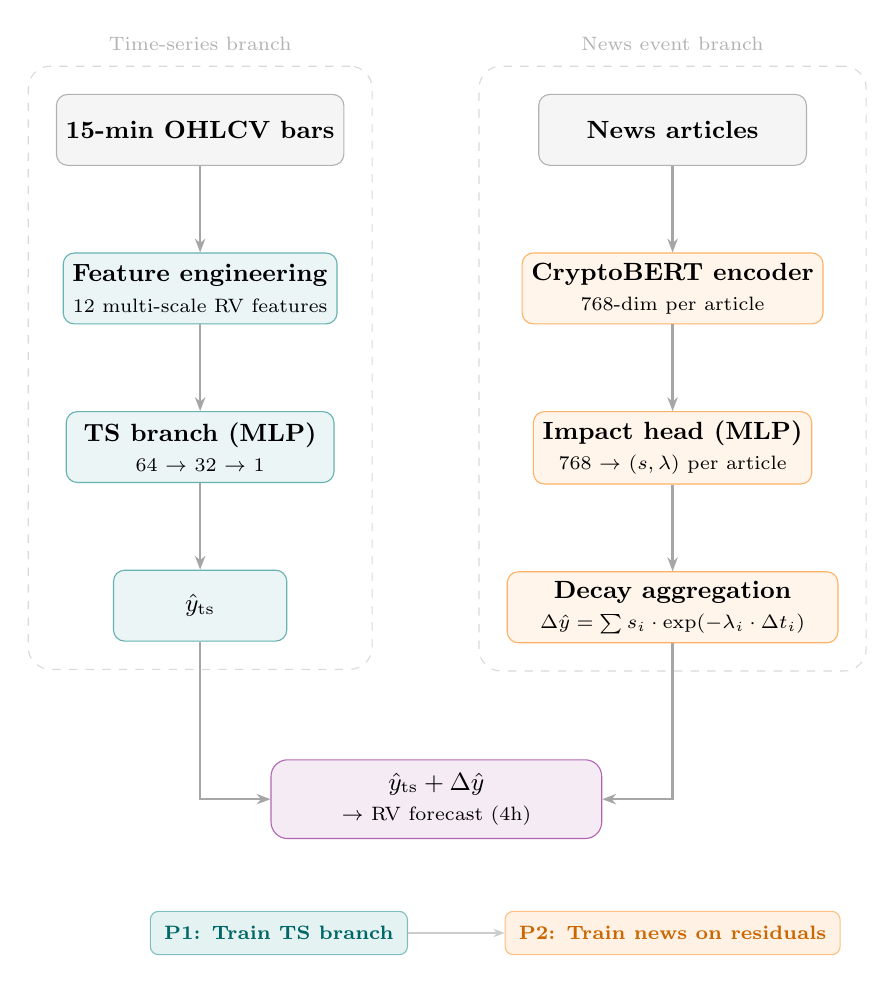
\begin{tikzpicture}[
    node distance=1.1cm,
    box/.style={rectangle, rounded corners=4pt, draw=gray!60, fill=gray!8, minimum height=0.9cm, minimum width=3.4cm, align=center, font=\small},
    tsbox/.style={rectangle, rounded corners=4pt, draw=teal!60, fill=teal!8, minimum height=0.9cm, minimum width=3.4cm, align=center, font=\small},
    newsbox/.style={rectangle, rounded corners=4pt, draw=orange!60, fill=orange!8, minimum height=0.9cm, minimum width=3.4cm, align=center, font=\small},
    outbox/.style={rectangle, rounded corners=6pt, draw=violet!60, fill=violet!8, minimum height=1cm, minimum width=4.2cm, align=center, font=\small},
    arr/.style={-{Stealth[length=5pt]}, gray!70, thick},
    dashedbox/.style={rectangle, rounded corners=8pt, draw=gray!30, dashed, inner sep=10pt},
    sublabel/.style={font=\scriptsize\color{gray!60}},
    phasebox/.style={rectangle, rounded corners=3pt, minimum height=0.55cm, align=center, font=\scriptsize\bfseries, inner sep=5pt},
]
% === Left branch (TS) at x=0 ===
\node[box] (input_ts) at (0,0) {\textbf{15-min OHLCV bars}};
\node[tsbox, below=of input_ts] (features) {\textbf{Feature engineering}\\\scriptsize 12 multi-scale RV features};
\node[tsbox, below=of features] (ts_mlp) {\textbf{TS branch (MLP)}\\\scriptsize 64 $\rightarrow$ 32 $\rightarrow$ 1};
\node[tsbox, below=of ts_mlp, minimum width=2.2cm] (yhat_ts) {$\hat{y}_{\text{ts}}$};
% === Right branch (News) at x=6 ===
\node[box] (input_news) at (6,0) {\textbf{News articles}};
\node[newsbox, below=of input_news] (cryptobert) {\textbf{CryptoBERT encoder}\\\scriptsize 768-dim per article};
\node[newsbox, below=of cryptobert] (impact) {\textbf{Impact head (MLP)}\\\scriptsize 768 $\rightarrow$ $(s, \lambda)$ per article};
\node[newsbox, below=of impact, minimum width=4.2cm] (decay) {\textbf{Decay aggregation}\\\scriptsize $\Delta\hat{y} = \sum s_i \cdot \exp(-\lambda_i \cdot \Delta t_i)$};
% === Output centered at x=3 ===
\node[outbox] (output) at (3,-8.5) {$\hat{y}_{\text{ts}} + \Delta\hat{y}$\\\scriptsize $\rightarrow$ RV forecast (4h)};
% === Arrows within TS branch ===
\draw[arr] (input_ts) -- (features);
\draw[arr] (features) -- (ts_mlp);
\draw[arr] (ts_mlp) -- (yhat_ts);
% === Arrows within News branch ===
\draw[arr] (input_news) -- (cryptobert);
\draw[arr] (cryptobert) -- (impact);
\draw[arr] (impact) -- (decay);
% === Arrows to output: L-bends entering from left and right ===
\draw[arr] (yhat_ts.south) |- (output.west);
\draw[arr] (decay.south) |- (output.east);
% === Dashed containers ===
\begin{scope}[on background layer]
\node[dashedbox, fit=(input_ts)(features)(ts_mlp)(yhat_ts)] (ts_container) {};
\node[dashedbox, fit=(input_news)(cryptobert)(impact)(decay)] (news_container) {};
\end{scope}
% === Branch labels ===
\node[sublabel, above=2pt of ts_container.north] {Time-series branch};
\node[sublabel, above=2pt of news_container.north] {News event branch};
% === Training phases (two phases only) ===
\node[phasebox, draw=teal!50, fill=teal!10, text=teal!80!black] (p1) at (1,-10.2) {P1: Train TS branch};
\node[phasebox, draw=orange!50, fill=orange!10, text=orange!80!black] (p2) at (6,-10.2) {P2: Train news on residuals};
\draw[gray!40, thick, -{Stealth[length=4pt]}] (p1.east) -- (p2.west);
\end{tikzpicture}
\caption{NED architecture. The time-series branch predicts $\hat{y}_{\text{ts}}$ from multi-scale realized volatility features. The news event branch compresses each article's CryptoBERT embedding into an impact scalar $s$ and decay rate $\lambda$, then aggregates them via exponential decay into a residual correction $\Delta\hat{y}$. The final forecast is their sum. Training proceeds in two phases: P1 trains the TS branch, and P2 trains the news branch on P1 residuals with the TS branch frozen.}
\label{fig:architecture}
\end{figure}


\begin{figure}[htbp]
\centering
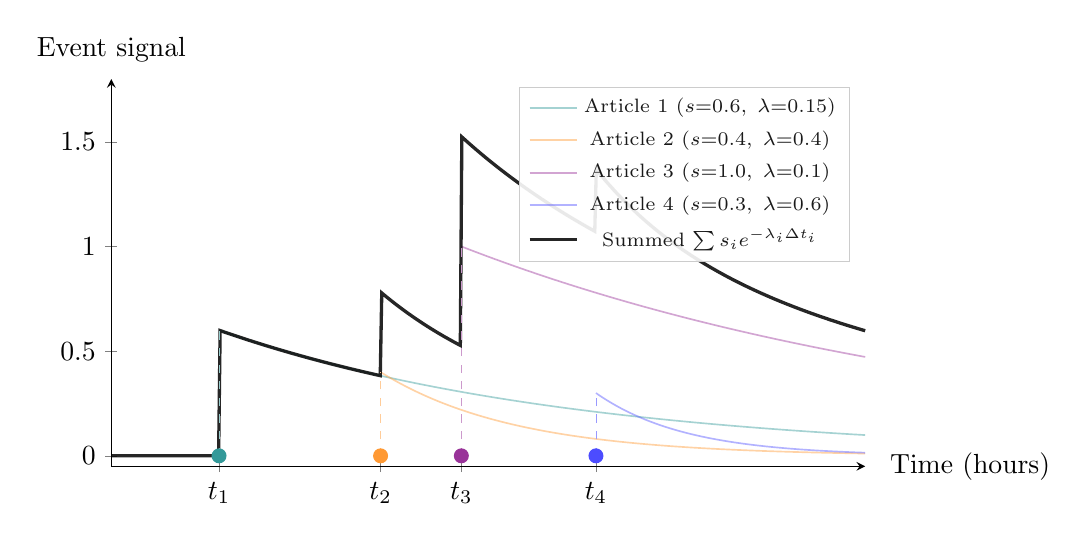
\begin{tikzpicture}
\begin{axis}[
    width=0.92\textwidth,
    height=6.5cm,
    xlabel={Time (hours)},
    ylabel={Event signal},
    xmin=0, xmax=14,
    ymin=-0.05, ymax=1.8,
    xtick={2,5,6.5,9},
    xticklabels={$t_1$, $t_2$, $t_3$, $t_4$},
    ytick={0,0.5,1.0,1.5},
    axis lines=left,
    every axis x label/.style={at={(ticklabel* cs:1.02)}, anchor=west},
    every axis y label/.style={at={(ticklabel* cs:1.02)}, anchor=south},
    legend style={
        at={(0.98,0.98)}, anchor=north east,
        font=\scriptsize, draw=gray!40,
        fill=white, fill opacity=0.9,
        row sep=1pt,
    },
    grid=none,
    clip=false,
]

% --- Individual decay curves (thin, colored) ---
\addplot[domain=2:14, samples=200, teal!70, semithick, opacity=0.5]
    {0.6 * exp(-0.15*(x-2))};
\addlegendentry{Article 1 ($s{=}0.6,\;\lambda{=}0.15$)}

\addplot[domain=5:14, samples=200, orange!70, semithick, opacity=0.5]
    {0.4 * exp(-0.4*(x-5))};
\addlegendentry{Article 2 ($s{=}0.4,\;\lambda{=}0.4$)}

\addplot[domain=6.5:14, samples=200, violet!70, semithick, opacity=0.5]
    {1.0 * exp(-0.1*(x-6.5))};
\addlegendentry{Article 3 ($s{=}1.0,\;\lambda{=}0.1$)}

\addplot[domain=9:14, samples=200, blue!60, semithick, opacity=0.5]
    {0.3 * exp(-0.6*(x-9))};
\addlegendentry{Article 4 ($s{=}0.3,\;\lambda{=}0.6$)}

% --- Summed signal (single expression using boolean conditions) ---
\addplot[domain=0:14, samples=500, black, very thick, opacity=0.85]
    { (x>=2)  * 0.6 * exp(-0.15*(x-2))
    + (x>=5)  * 0.4 * exp(-0.4*(x-5))
    + (x>=6.5)* 1.0 * exp(-0.1*(x-6.5))
    + (x>=9)  * 0.3 * exp(-0.6*(x-9))
    };
\addlegendentry{Summed $\sum s_i e^{-\lambda_i \Delta t_i}$}

% --- Article arrival markers on x-axis ---
\addplot[only marks, mark=*, mark size=2.5pt, teal!80, forget plot] coordinates {(2,0)};
\addplot[only marks, mark=*, mark size=2.5pt, orange!80, forget plot] coordinates {(5,0)};
\addplot[only marks, mark=*, mark size=2.5pt, violet!80, forget plot] coordinates {(6.5,0)};
\addplot[only marks, mark=*, mark size=2.5pt, blue!70, forget plot] coordinates {(9,0)};

% --- Dashed vertical lines at arrivals ---
\draw[teal!40, dashed, very thin] (axis cs:2,0) -- (axis cs:2,0.6);
\draw[orange!40, dashed, very thin] (axis cs:5,0) -- (axis cs:5,0.4);
\draw[violet!40, dashed, very thin] (axis cs:6.5,0) -- (axis cs:6.5,1.0);
\draw[blue!40, dashed, very thin] (axis cs:9,0) -- (axis cs:9,0.3);

\end{axis}
\end{tikzpicture}
\caption{Event signal accumulation. Each news article contributes an exponentially decaying signal with learned magnitude $s_i$ and decay rate $\lambda_i$. The total event signal (black) is the sum of all active decays at each time step. Articles with large $s$ and small $\lambda$ (e.g., Article~3) produce persistent signals, while articles with small $s$ and large $\lambda$ (e.g., Article~4) vanish quickly. The signal spikes at each article arrival and decays between arrivals, resembling a Hawkes-type self-exciting process with content-dependent kernels.}
\label{fig:decay_stacking}
\end{figure}

% Section 3.2 NED Architecture

\newpage
\subsection{NED architecture}
\label{sec:architecture}

The News Event Decay (NED) model decomposes the volatility forecast into two additive components: a time-series prediction and a news-driven residual correction. Figure~\ref{fig:architecture} illustrates the full architecture. Let $\hat{y}_t$ denote the final log-RV forecast at bar $t$. The model produces
\begin{equation}
    \hat{y}_t = \hat{y}_t^{\text{ts}} + \Delta\hat{y}_t^{\text{news}},
    \label{eq:residual}
\end{equation}
where $\hat{y}_t^{\text{ts}}$ is the output of the time-series branch and $\Delta\hat{y}_t^{\text{news}}$ is the correction from the news event branch. This residual architecture ensures a clean separation of roles: the time-series branch captures the baseline volatility dynamics, and the news branch models only what the time-series features cannot explain.

\subsubsection{Time-series branch}

The time-series branch maps the 12-dimensional feature vector $\mathbf{x}_t$ 
(described in Table~\ref{tab:ts_features}) to a scalar volatility forecast 
through a two-layer feedforward network with ReLU activations. This 
architecture can be interpreted as a nonlinear generalization of the HAR 
model: the multi-scale realized variance inputs ($\text{rv}_4$, 
$\text{rv}_{16}$, $\text{rv}_{96}$, $\text{rv}_{384}$) correspond to the 
HAR components at different aggregation scales \citep{Corsi_2008}, while the 
MLP allows for nonlinear interactions among these scales and auxiliary 
features such as volume, skewness, and kurtosis.

\subsubsection{News event branch}

The news event branch processes all articles published within a 12-hour lookback window preceding bar $t$. Let $\{a_1, \ldots, a_K\}$ denote these articles, where each article $a_k$ has a pre-computed CryptoBERT embedding $\mathbf{e}_k \in \mathbb{R}^{768}$ and publication timestamp $\tau_k$. For each article, a small feedforward network produces two scalar parameters:
\begin{equation}
    (s_k, \lambda_k) = h(\mathbf{e}_k; \psi),
    \label{eq:impact_head}
\end{equation}
where $h(\cdot; \psi)$ is a two-layer MLP parameterized by $\psi$. The impact magnitude $s_k = \text{Softplus}(\tilde{s}_k)$ is constrained to be strictly positive, capturing the strength of the article's effect on volatility. The decay rate $\lambda_k = \text{Softplus}(\tilde{\lambda}_k)$ governs how quickly this effect dissipates over time.

The news event signal at bar $t$ aggregates all articles in the lookback window via exponential decay:
\begin{equation}
    \Delta\hat{y}_t^{\text{news}} = \sum_{k=1}^{K} s_k \cdot \exp(-\lambda_k \cdot \Delta t_k),
    \label{eq:decay}
\end{equation}
where $\Delta t_k = t - \tau_k$ is the elapsed time (in minutes) since article $a_k$ was published. This formulation is inspired by the kernel structure of Hawkes processes \citep{HAWKES1971}, in which past events excite future intensity through decaying kernels. A critical distinction is that in our framework, both the excitation magnitude and the decay rate are conditioned on article content through the CryptoBERT embedding, rather than being fixed parameters shared across all events. This allows the model to learn, for instance, that regulatory news produces a large, slowly decaying signal while routine market commentary produces a small, rapidly decaying one.

Each article is compressed to just two scalars $(s_k, \lambda_k)$, making the news branch interpretable: for any given forecast, one can identify exactly which articles contributed, by how much, and for how long. Figure~\ref{fig:decay_stacking} illustrates how individual article decays stack additively into the aggregate event signal.

\subsubsection{Residual combination}

The final forecast is the direct sum of the two branches (Equation~\ref{eq:residual}). Unlike concatenation-based fusion architectures common in multimodal learning, the additive structure offers three advantages. First, the contribution of news to any individual forecast is directly readable as $\Delta\hat{y}_t^{\text{news}}$, requiring no post-hoc attribution. Second, the news branch cannot suppress or override the time-series signal; it can only adjust it. Third, the residual design prevents the gradient suppression problem that arises in concatenation architectures, where a strong time-series representation causes the fusion layer to ignore the weaker news signal during joint training.

We note that $\Delta\hat{y}_t^{\text{news}}$ is permitted to only positive corrections which indicate that news increases expected volatility beyond the time-series baseline,

% Section 3.3 Training Procedure

\subsection{Training procedure}
\label{sec:training}

The model is trained in two sequential phases to ensure that the news branch learns to correct the time-series model's errors rather than redundantly modeling dynamics already captured by the time-series features. All phases minimize mean squared error on log-transformed realized volatility, $y_t = \log(\text{RV}_{t,H} + \epsilon)$:
\begin{equation}
    \mathcal{L} = \frac{1}{N} \sum_{t=1}^{N} 
    \left( y_t - \hat{y}_t^{\text{ts}} - \Delta\hat{y}_t^{\text{news}} \right)^2.
    \label{eq:loss}
\end{equation}
In Phase~1, only the time-series branch is trained, with $\Delta\hat{y}_t^{\text{news}} = 0$, establishing a strong baseline based solely on market dynamics. In Phase~2, the time-series branch is frozen and the news branch is trained to predict the residual component left unexplained by the Phase~1 model. This design forces the news branch to capture incremental information from textual signals rather than relearning patterns already represented by the time-series branch. The staged protocol follows a logic analogous to gradient boosting \citep{Friedman_2001}, where subsequent learners target the residuals of earlier learners. Table~\ref{tab:training_phases} summarizes the configuration of each phase.

\begin{table}[htbp]
\centering
\caption{Training phase configuration}
\label{tab:training_phases}
\small
\begin{tabular}{@{}lcc@{}}
\toprule
 & Phase 1 & Phase 2 \\
\midrule
TS branch & trained & frozen \\
News branch & frozen & trained \\
Learning rate & $10^{-4}$ & $10^{-4}$ \\
\bottomrule
\end{tabular}
\end{table}

We use AdamW \citep{adamw} with a batch size of 64 and early stopping with a patience of 15 epochs throughout both phases. No joint fine-tuning phase is applied, so the final prediction preserves the residual-correction structure in which the news branch contributes only an additive adjustment to the fixed time-series baseline.

\subsubsection{Expanding window evaluation}

To assess out-of-sample performance under realistic conditions, we employ an expanding window protocol. For each evaluation window, the model is trained using all data available before the validation period. The subsequent six months are used for validation, and the next six months are held out as the test set. The training set grows monotonically across windows, allowing the model to incorporate newly observed market regimes while being evaluated only on strictly unseen future data. The full two-phase training procedure is re-executed from scratch for each window to prevent information leakage.


\subsection{Baselines}
\label{sec:baselines}

We compare NED against four baseline models that span the standard 
approaches to realized volatility forecasting. The first two are classical 
econometric models that do not use news, the third is a parametric model 
augmented with the same news residual as NED, and the fourth is a neural 
time-series model that uses the same realized-variance features as NED 
without the news branch.

\subsubsection{HAR}

The heterogeneous autoregressive model of \citet{Corsi_2008} forecasts 
log-realized variance as a linear combination of realized variance 
averaged over multiple frequencies. The original HAR specification uses 
daily, weekly, and monthly aggregates motivated by the heterogeneous 
trading horizons of equity market participants. We adapt this 
specification to the high-frequency cryptocurrency setting by using four 
trailing realized-variance components computed over 4, 16, 96, and 384 
bars at 15-minute resolution, corresponding to 1-hour, 4-hour, 24-hour, 
and 4-day windows:
\begin{equation}
    \hat{y}_t^{\text{HAR}} = \beta_0 
    + \beta_1 \, \text{rv}_4 
    + \beta_2 \, \text{rv}_{16} 
    + \beta_3 \, \text{rv}_{96} 
    + \beta_4 \, \text{rv}_{384}.
    \label{eq:har}
\end{equation}
The four aggregation scales match the realized-variance features used in 
the time-series branch of NED (Table~\ref{tab:ts_features}), so that 
the HAR baseline differs from TS-only only in functional form. HAR is 
linear in the four scale-specific realized variances, while TS-only 
maps the same features through a two-layer nonlinear network. The 
coefficients are estimated by ordinary least squares on the training 
portion of each expanding window and held fixed during the out-of-sample 
evaluation. This adapted specification preserves the multi-scale 
aggregation logic of HAR while accommodating the absence of a natural 
daily unit in twenty-four-hour cryptocurrency markets.

\subsubsection{EGARCH}

The exponential GARCH model of \citet{Nelson_1991} captures asymmetric 
volatility responses through a logarithmic specification of the conditional 
variance:
\begin{equation}
    \log \sigma_t^2 = \omega + \alpha \frac{|r_{t-1}|}{\sigma_{t-1}} 
    + \gamma \frac{r_{t-1}}{\sigma_{t-1}} + \beta \log \sigma_{t-1}^2,
    \label{eq:egarch}
\end{equation}
where $\gamma$ permits negative return shocks to elevate volatility more 
than positive shocks of equal magnitude, capturing the leverage effect 
documented in equity and increasingly in cryptocurrency markets. We 
estimate the EGARCH(1,1) specification by quasi-maximum likelihood on 
15-minute log returns within each expanding window's training set, and 
produce out-of-sample volatility forecasts by iterating the conditional 
variance equation forward over the relevant horizon. The forecast is 
converted to log-RV by summing the conditional variances over the $H$ 
bars in the forecast window.

\subsubsection{EGARCH+NED}

The EGARCH+NED hybrid replaces the neural time-series branch of NED with 
the EGARCH forecast described above while retaining the per-article 
learned news residual:
\begin{equation}
    \hat{y}_t^{\text{EGARCH+NED}} = \hat{y}_t^{\text{EGARCH}} 
    + \Delta\hat{y}_t^{\text{news}}.
    \label{eq:egarch_ned}
\end{equation}
The news branch is trained to predict the residual $y_t - 
\hat{y}_t^{\text{EGARCH}}$ from the article-level CryptoBERT embeddings, 
following the same two-phase protocol described in 
Section~\ref{sec:training}. This baseline isolates the contribution of 
the time-series component by holding the news mechanism fixed and 
varying only the underlying volatility model. A comparison between NED 
and EGARCH+NED reveals the extent to which the news residual interacts 
with the flexibility of the time-series model, while a comparison between 
EGARCH+NED and standalone EGARCH reveals the marginal value of news 
when added to a fixed parametric backbone.

\subsubsection{TS-only}

The TS-only baseline is the time-series branch of NED trained on its own, 
with the news residual constrained to zero throughout training and 
evaluation. It uses the same 12-dimensional feature set, the same 
two-layer feedforward architecture, the same expanding-window protocol, 
and the same loss function as the full NED model. The only difference is 
that no news information is available. TS-only therefore measures the 
forecast value obtainable from realized-variance features alone under a 
neural architecture, isolating the marginal contribution of news in the 
comparison against NED.

\subsection{Evaluation metrics and statistical tests}
\label{sec:metrics}

We evaluate forecast accuracy on four metrics that capture distinct 
aspects of volatility forecasting performance. Each metric is computed on 
the out-of-sample test bars within each expanding window and then pooled 
across windows for the summary tables. Per-window decompositions appear 
in the appendix.

\subsubsection{Coefficient of determination}

The out-of-sample $R^2$ is computed against the variance of the 
log-realized-volatility series in the test set:
\begin{equation}
    R^2 = 1 - \frac{\sum_t (y_t - \hat{y}_t)^2}{\sum_t (y_t - \bar{y})^2},
    \label{eq:r2}
\end{equation}
where $\bar{y}$ is the in-sample mean of $y_t$ on the training set. 
Negative values indicate that the model performs worse than a 
constant-mean forecast, a possibility that arises for misspecified models 
on the log-transformed target.

\subsubsection{Directional accuracy}

The directional accuracy metric measures the fraction of bars at which 
the forecast and the realized volatility move in the same direction 
relative to their respective previous values:
\begin{equation}
    \text{DA} = \frac{1}{N} \sum_{t=1}^{N} \mathbf{1}\!\left\{ 
    \text{sign}(\text{RV}_t - \text{RV}_{t-1}) = 
    \text{sign}(\widehat{\text{RV}}_t - \widehat{\text{RV}}_{t-1}) 
    \right\}.
    \label{eq:da}
\end{equation}
DA is computed on the original RV scale rather than the log scale, 
making it interpretable as the accuracy of binary up-or-down classification.

\subsubsection{QLIKE}

The QLIKE loss function of \citet{Patton_2011} is a quasi-likelihood 
metric robust to noise in the realized variance proxy:
\begin{equation}
    \text{QLIKE} = \frac{1}{N} \sum_{t=1}^{N} \left( 
    \frac{\text{RV}_t}{\widehat{\text{RV}}_t} - 
    \log \frac{\text{RV}_t}{\widehat{\text{RV}}_t} - 1 \right).
    \label{eq:qlike}
\end{equation}
QLIKE penalizes underprediction of high volatility more heavily than 
overprediction of an equal proportional magnitude, making it especially 
informative for risk management applications where missing a volatility 
spike is costlier than a false alarm. \citet{Patton_2011} shows that 
QLIKE is one of only two loss functions (the other being MSE on level 
RV) that produce consistent forecast rankings when the realized variance 
is an unbiased but noisy proxy of the latent integrated variance, and 
recommends QLIKE in particular because of its lower sensitivity to 
proxy noise.

\subsubsection{Mean squared error}

MSE is computed on the log-RV scale rather than on RV levels:
\begin{equation}
    \text{MSE} = \frac{1}{N} \sum_{t=1}^{N} (y_t - \hat{y}_t)^2.
    \label{eq:mse}
\end{equation}
Computing MSE on log-RV places equal weight on proportional forecast 
errors at high and low volatility regimes, while MSE on the level would 
be dominated by errors during high-volatility periods.

\subsubsection{Diebold-Mariano test with small-sample correction}

To assess whether forecast improvements are statistically significant, 
we apply the \citet{DM_1995} test with the \citet{Harvey_1997} 
small-sample correction. Given two competing forecasts with loss series 
$L_t^{(1)}$ and $L_t^{(2)}$, the test evaluates the null hypothesis that 
the expected loss differential $d_t = L_t^{(1)} - L_t^{(2)}$ is zero. 
The test statistic is
\begin{equation}
    \text{DM}^* = \sqrt{\frac{N + 1 - 2h + h(h-1)/N}{N}} \cdot 
    \frac{\bar{d}}{\sqrt{\widehat{\text{Var}}(\bar{d})}},
    \label{eq:dm}
\end{equation}
where $\bar{d}$ is the sample mean of the loss differential, 
$\widehat{\text{Var}}(\bar{d})$ is the Newey-West variance estimator with 
$h - 1$ lags, $h$ is the forecast horizon in bars, and $N$ is the number 
of test bars. \citet{Harvey_1997} show that comparing DM$^*$ to a 
Student-$t$ distribution with $N - 1$ degrees of freedom corrects the 
size distortion of the standard DM test at finite sample sizes. We 
report two-sided $p$-values for the DM$^*$ test on both QLIKE and MSE 
loss differentials between NED and TS-only. Tests for other model 
comparisons follow the same protocol.

\newpage

\section{Results}\label{sec:results}


\subsection{Main Results}

 
% Requires: \usepackage{booktabs, multirow}

\begin{table}[htbp]
\centering
\caption{Out-of-Sample Forecast Performance (Pooled Expanding Windows)}
\label{tab:forecast_summary}
\small
\setlength{\tabcolsep}{5pt}
\textit{Panel A: 1-Hour RV}

\vspace{0.3em}
\begin{tabular}{@{}c|c| cccc@{}}
\toprule
Asset & Model & $R^2$ & DA & QLIKE & MSE \\
\midrule
\multirow{5}{*}{\textbf{BTC}}
 & HAR           & $-$0.139 & 0.508 & 1.136 & 2.338 \\
 & EGARCH        & 0.050 & 0.634 & 0.792 & 1.914 \\
 & EGARCH+NED    & 0.337 & 0.703 & 1.133 & 1.336 \\
 & TS-only       & 0.419 & 0.732 & 0.955 & 1.169 \\
 & NED           & 0.427 & 0.734 & 0.917$^{***}$\,($-$3.9\%) & 1.154$^{***}$\,($-$1.3\%) \\[4pt]\hline
\end{tabular}
\vspace{1.5em}

\textit{Panel B: 4-Hour RV}

\vspace{0.3em}
\begin{tabular}{@{}c|c| cccc@{}}
\toprule
Asset & Model & $R^2$ & DA & QLIKE & MSE \\
\midrule
\multirow{5}{*}{\textbf{BTC}}
 & HAR           & $-$0.232 & 0.500 & 0.711 & 1.769 \\
 & EGARCH        & 0.191 & 0.661 & 0.576 & 1.127 \\
 & EGARCH+NED    & 0.333 & 0.697 & 0.707 & 0.929 \\
 & TS-only       & 0.421 & 0.715 & 0.605 & 0.807 \\
 & NED           & 0.441 & 0.726 & 0.571$^{***}$\,($-$5.6\%) & 0.779$^{***}$\,($-$3.5\%) \\[4pt]\hline
\noalign{\vspace{4pt}}
\end{tabular}
\vspace{0.5em}
\begin{minipage}{\textwidth}
\footnotesize
\textit{Notes:} Results averaged across six expanding windows (Jan 2023--Dec 2025). $R^2$ and MSE are computed on log-transformed realized volatility; QLIKE and DA are computed on levels. QLIKE and MSE for the NED row show percentage change relative to TS-only in parentheses (negative = improvement). $^{*}p<0.10$, $^{**}p<0.05$, $^{***}p<0.01$ from DM test with \citet{Harvey_1997} small-sample correction. Per-window results in Tables~\ref{tab:expanding_btc}.
\end{minipage}
\end{table}
\newpage

Table~\ref{tab:forecast_summary} reports out-of-sample forecast performance 
for the four baseline models and the two news-augmented variants on 
Bitcoin at the 1-hour and 4-hour horizons. Each row pools forecasts 
across the six expanding-window test periods from January 2023 through 
December 2025. Per-window results are reported in Appendix 
Table~\ref{tab:expanding_btc}.

We begin with the baseline comparison among models that do not use news. 
The HAR model performs poorly at both horizons, with negative $R^2$ 
values indicating that its forecasts are worse than a constant-mean 
predictor on log-RV. This result is not unusual at intraday horizons in 
high-frequency cryptocurrency data. HAR was designed for daily 
volatility forecasting in equity markets, where the trading day provides 
a natural unit of aggregation, and the absence of such a unit on 
twenty-four-hour cryptocurrency markets weakens its multi-scale 
aggregation structure. EGARCH improves substantially on HAR, recovering 
positive $R^2$ at both horizons. The TS-only model, which uses the same 
12-dimensional feature set as the time-series branch of NED but is 
trained end-to-end without the news residual, outperforms both classical 
baselines by a wide margin. At the 4-hour horizon, TS-only achieves 
$R^2 = 0.421$ compared with $0.191$ for EGARCH and $-0.232$ for HAR. The 
TS-only model establishes a strong benchmark against which the 
news-augmented NED model must demonstrate value.

Adding the news residual to the neural time-series branch produces 
statistically significant gains at both horizons on QLIKE and MSE. At 
the 4-hour horizon, NED reduces QLIKE by 5.6\% and MSE by 3.5\% relative 
to TS-only, with both improvements significant at the 1\% level under 
the Diebold-Mariano test using the \citet{Harvey_1997} small-sample 
correction. At the 1-hour horizon the QLIKE improvement is 3.9\% and the 
MSE improvement is 1.3\%, again with $p < 0.01$ on both losses. The 
directional accuracy and $R^2$ are largely unchanged. News information 
sharpens the magnitude of the volatility forecast without altering its 
directional component, which is the expected result given that TS-only 
already captures regime direction from the multi-scale realized-variance 
features.

The contribution of news to volatility forecasts is most clearly 
illustrated by comparing NED to its parametric counterpart, EGARCH+NED. 
This hybrid uses the same news residual but adds it to an EGARCH 
forecast rather than to the neural time-series branch, providing a 
useful diagnostic for how much information news adds to baselines of 
different quality. Relative to standalone EGARCH at the 4-hour horizon, 
the news residual raises $R^2$ from 0.191 to 0.333, improves directional 
accuracy from 0.661 to 0.697, and reduces MSE by 17.6\%. The same 
pattern holds at the 1-hour horizon, where $R^2$ rises from 0.050 to 
0.337 and MSE falls by 30.2\%. In proportional terms these improvements 
are an order of magnitude larger than the corresponding improvements 
from TS-only to NED. The pattern is consistent with a simple 
interpretation: news contributes more forecast value to a weaker 
baseline because there is more residual information for it to capture. 
A parametric volatility recursion such as EGARCH absorbs new information 
at a fixed rate determined by its conditional variance equation. A 
neural time-series branch, in contrast, processes multi-scale 
realized-variance features in parallel and internalizes regime shifts 
more quickly, leaving less unexplained variation for the news residual 
to exploit. The EGARCH+NED result therefore demonstrates that the news 
residual carries genuine forecast value: it improves any baseline to 
which it is added, and the magnitude of the improvement scales with the 
information lag of the underlying model.

The one exception is QLIKE, which worsens under EGARCH+NED relative to 
EGARCH (0.707 versus 0.576 at the 4-hour horizon, and 1.133 versus 0.792 
at the 1-hour horizon). QLIKE penalizes underprediction of high 
volatility more heavily than overprediction, and the deterioration 
indicates that the news adjustment occasionally moves EGARCH's 
high-volatility forecasts in the wrong direction. The full NED model 
does not exhibit this trade-off: at both horizons, QLIKE and MSE improve 
simultaneously against TS-only. The joint training of the time-series 
branch and the news branch under a common loss function calibrates the 
news adjustment against the actual residual structure of the 
time-series predictions, which is not the case when news is added to a 
pre-estimated parametric model. This is the central architectural 
distinction between EGARCH+NED and NED, and it explains why a single 
news mechanism can produce divergent QLIKE and MSE responses depending 
on how it is integrated into the volatility model.

Two final observations close the main results discussion. First, the 
forecast improvement from NED is concentrated in QLIKE rather than 
$R^2$ at both horizons, with MSE gains positive but smaller. The 
practical implication is that NED improves the quality of 
high-volatility forecasts, which is precisely the regime in which 
volatility forecasts are most valuable for risk management, derivatives 
pricing, and dynamic position sizing. A model that better identifies 
imminent volatility expansions is more useful than one that improves 
marginally on routine low-volatility forecasts. Second, the gap between 
TS-only and NED is consistent across the six expanding windows. The 
QLIKE improvement is positive in all six windows and statistically 
significant at the 1\% level in all six of them. The robustness of the 
gain across distinct market regimes, including the bear market period 
of 2023 H1 and the ETF-driven rally of 2024 H1, suggests that the 
contribution of news to high-frequency volatility forecasts is not 
concentrated in any single macro environment.
\subsection{Z-score analysis}
\begin{table}[htbp]
\centering
\caption{Forecast performance by volatility decile (4-Hour RV, BTC)}
\label{tab:decile_performance}
\small
\setlength{\tabcolsep}{6pt}
\begin{tabular}{@{}c c c c c c c c@{}}
\toprule
 & & \multicolumn{2}{c}{$R^2$} & & \multicolumn{2}{c}{\% improvement} \\
\cmidrule(lr){3-4} \cmidrule(lr){6-7}
Decile & $\bar{z}$ & TS-only & NED & $\Delta R^2$ & QLIKE & MSE \\
\midrule
1 (low)   & $-$2.22 & $-$0.147 & $-$0.080 & 0.067 & $-$7.7 & $-$5.9 \\
2         & $-$0.92 &    0.622 &    0.632 & 0.010 & $-$6.4 & $-$2.7 \\
3         & $-$0.54 &    0.550 &    0.560 & 0.010 & $-$2.7 & $-$2.2 \\
4         & $-$0.28 &    0.464 &    0.479 & 0.015 & $-$3.8 & $-$2.8 \\
5         & $-$0.07 &    0.390 &    0.409 & 0.019 & $-$4.0 & $-$3.1 \\
6         &    0.13 &    0.417 &    0.437 & 0.020 & $-$4.0 & $-$3.4 \\
7         &    0.34 &    0.458 &    0.470 & 0.012 & $-$3.0 & $-$2.2 \\
8         &    0.59 &    0.500 &    0.508 & 0.007 & $-$3.0 & $-$1.5 \\
9         &    0.97 &    0.576 &    0.577 & 0.001 & $-$3.6 & $-$0.2 \\
10 (high) &    2.31 & $-$0.280 & $-$0.217 & 0.063 & $-$5.9 & $-$4.9 \\
\bottomrule
\end{tabular}
\vspace{0.5em}
\begin{minipage}{\textwidth}
\footnotesize
\textit{Notes:} Pooled out-of-sample observations are sorted into deciles by the realized volatility $z$-score (standardized within each expanding window). $\bar{z}$ is the within-decile mean. Each decile contains 10,464--10,465 observations. $R^2$ is computed on log-transformed realized volatility; $\Delta R^2$ is the NED gain over TS-only. QLIKE and MSE columns report percentage improvement of NED over TS-only (negative = improvement); QLIKE is computed on levels and MSE on log-RV.
\end{minipage}
\end{table}


\section{Economic Interpretation}
\label{sec:economic}

The advantage of the NED framework over a black-box deep learning forecast is that the learned parameters $(s_k, \lambda_k)$ admit a direct economic interpretation. The impact magnitude $s_k$ measures the contribution of article $k$ to the residual log-volatility forecast at the moment of publication, and the decay rate $\lambda_k$ governs how quickly that contribution dissipates. This section examines whether these learned quantities exhibit the cross-sectional and temporal structure that economic reasoning would predict. We organize the analysis around three questions corresponding to our central research question: how long does news move volatility (Section~\ref{sec:timescale}), how does news content shape the impact (Section~\ref{sec:categories}), and what dimension of the text representation does the model actually use (Section~\ref{sec:sentiment}).

\subsection{Timescale: How long does news move volatility?}
\label{sec:timescale}

\begin{figure}[htbp]
\centering
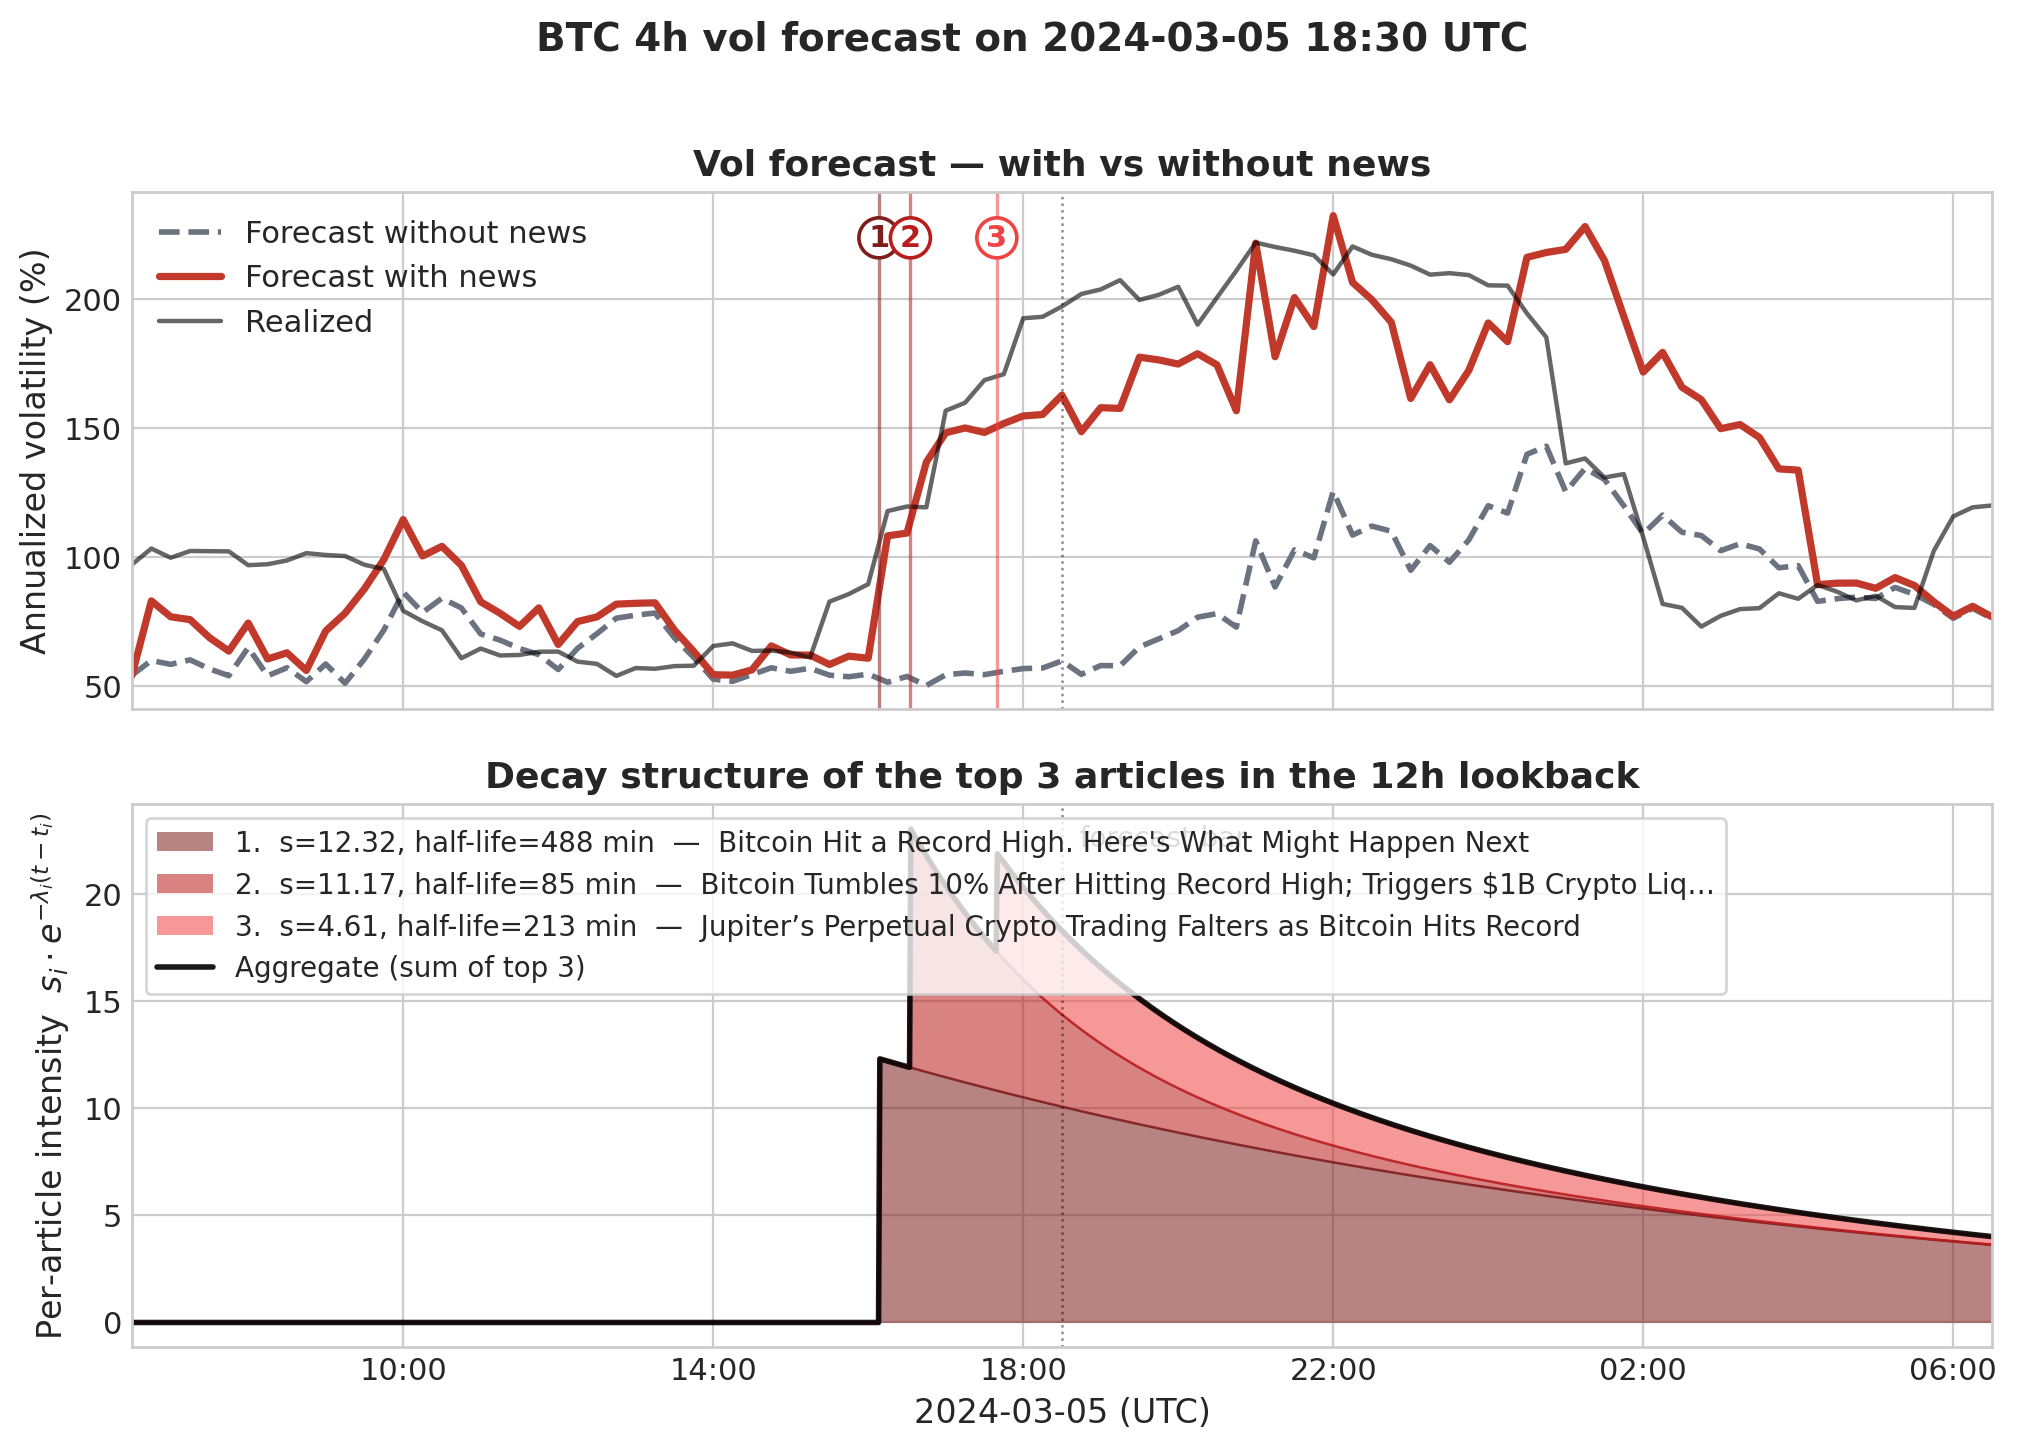
\includegraphics[width=\textwidth]{figures/casestudy.png}
\caption{News-driven forecast adjustment around the Bitcoin all-time high of 5 March 2024. 
The upper panel compares the 4-hour annualized realized volatility (gray) with two 
forecasts: the time-series-only baseline (dashed) and the full NED model (red). 
Three articles publishing during the build-up phase, indicated by vertical markers in 
the upper panel and labelled 1--3 in the lower panel, drive the forecast separation. 
The lower panel reports the learned per-article decay structure $s_k \exp(-\lambda_k (t - t_k))$ 
for each of these articles, together with their aggregate. Half-lives are reported in 
the legend and differ substantially across the three articles, with the forward-looking 
analysis of the new high persisting roughly an order of magnitude longer than the 
post-event report on the subsequent decline.}
\label{fig:casestudy}
\end{figure}


Figure~\ref{fig:casestudy} presents a single forecasting episode that illustrates how the news branch reshapes the 4-hour BTC volatility forecast. On 5 March 2024, Bitcoin reached an all-time high before retracing roughly 10\% within several hours, triggering more than one billion dollars in derivatives liquidations. Three articles arrived during the build-up phase, summarized in the lower panel of Figure~\ref{fig:casestudy}: a forward-looking analysis of the new record, a report on the subsequent decline and the liquidations it produced, and a derivatives-platform incident report. The model learns markedly different decay profiles across these articles. The forward-looking article carries the longest half-life at 488 minutes, the post-event report decays within 85 minutes, and the platform incident sits in between at 213 minutes. The aggregate signal in the lower panel translates into the upward shift visible in the forecast in the upper panel, which tracks realized volatility substantially better than the time-series-only baseline. The episode is illustrative rather than representative, but it demonstrates that the per-article parameters perform economically interpretable work. Anticipatory content persists longer than backward-looking commentary, and the forecast separation from the baseline is driven by a small number of high-impact articles.


\begin{figure}[htbp]
\centering
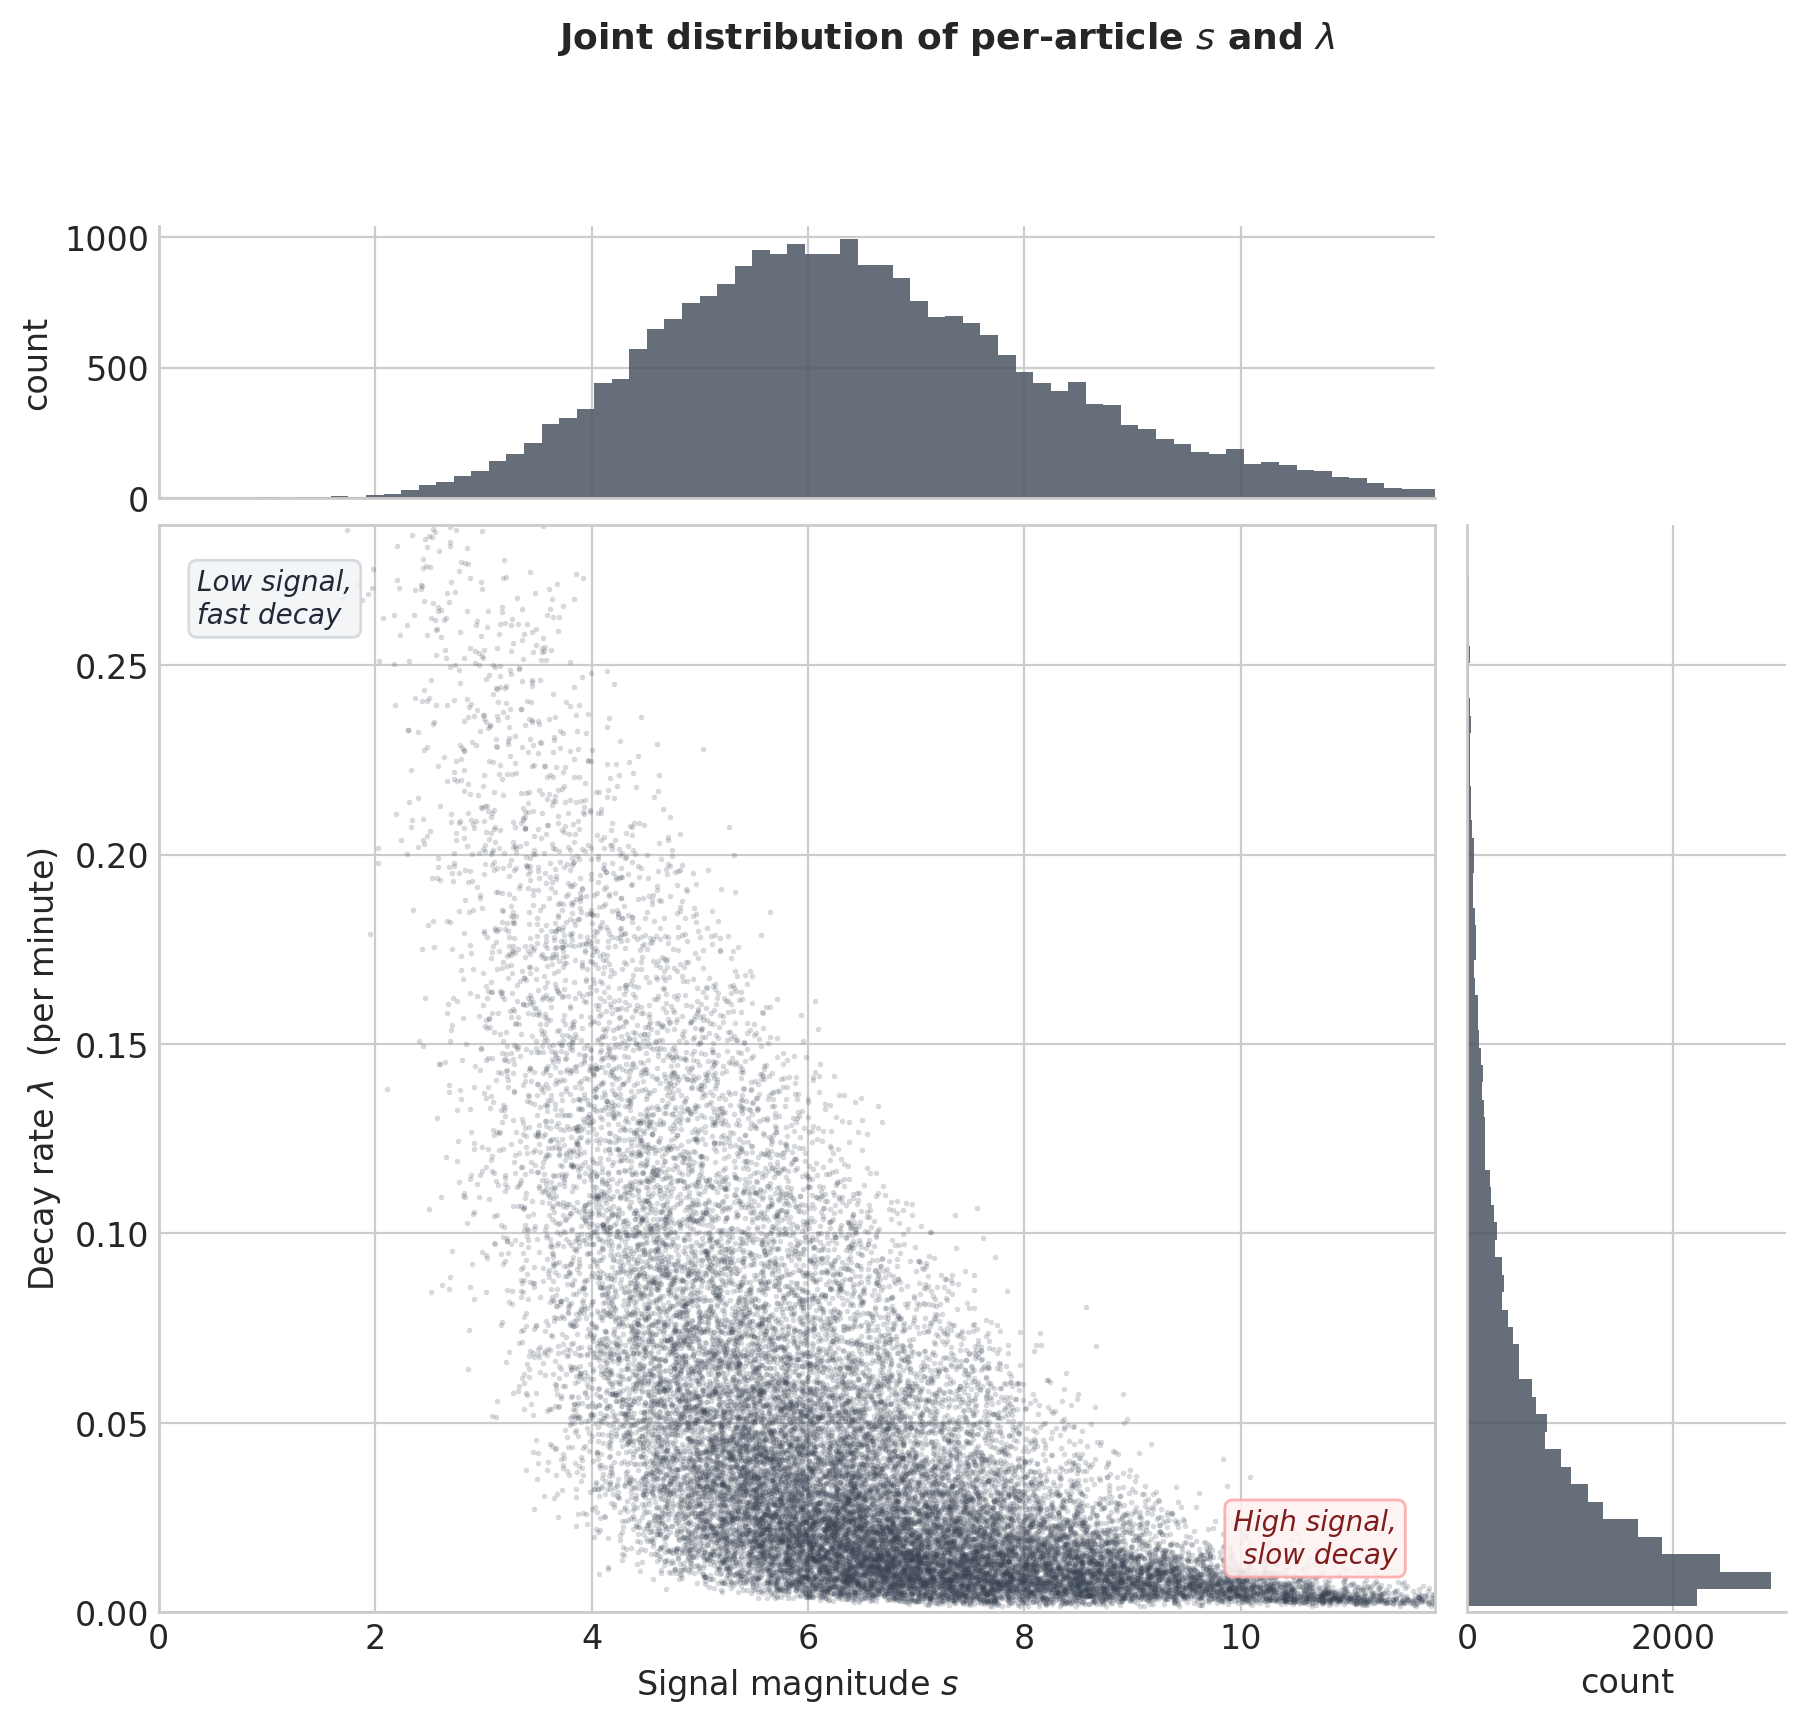
\includegraphics[width=0.85\textwidth]{figures/distribution.png}
\caption{Joint distribution of the per-article impact magnitude $s$ and decay rate 
$\lambda$ learned by the NED news branch. Each point corresponds to one article 
appearing in the test set of one of the six BTC 4-hour expanding windows. The marginal 
distributions are reported on the top and right axes. The impact magnitude is right-skewed 
with a mode near $s \approx 3.5$ and a long tail. The decay rate is concentrated at 
small values, with the bulk of the mass corresponding to half-lives between 30 minutes 
and three hours. The joint scatter shows a clear negative association between $s$ and 
$\lambda$: articles with the largest learned impacts cluster in the slow-decay region 
(high signal, slow decay), while articles with weak signals decay rapidly (low signal, 
fast decay). The pattern is not imposed by the architecture, which produces $s$ and 
$\lambda$ as independent outputs of the same MLP.}
\label{fig:joint}
\end{figure}

To assess whether this pattern holds in aggregate, we extract the learned 
$(s_k, \lambda_k)$ for every article entering every test-period forecast 
across the six expanding windows, yielding $25{,}231$ article-level 
parameter pairs. Figure~\ref{fig:joint} reports the joint distribution. 
The marginal distribution of impact magnitudes is right-skewed with a mode 
near $s = 5\text{–}6$ and a long tail extending past $s = 10$, consistent 
with the heavy-tailed nature of news-driven volatility shocks. The marginal 
distribution of decay rates is concentrated at small values. The median 
$\lambda$ corresponds to a half-life of approximately 30 minutes, and the 
interquartile range spans roughly 15 to 70 minutes. Half-lives exceeding 
four hours account for less than 5\% of articles.

A clear negative association between $s$ and $\lambda$ is visible in the joint scatter. Articles with the largest impact magnitudes concentrate in the slow-decay region, while articles with weak signal tend to decay rapidly. The pattern is not imposed by the architecture. The news branch produces $s$ and $\lambda$ as two independent outputs of the same MLP, with no parametric coupling between them in the forward pass. The observed structure therefore reflects what the model has learned from the data, namely that strong shocks tend to be absorbed slowly while weak shocks fade quickly. Combinations such as a strong but short-lived signal or a weak but persistent one remain feasible under the architecture, but the dominant pattern places the highest-impact news in a long-persistence regime.

\subsection{News category and impact heterogeneity}
\label{sec:categories}

To examine whether the learned news impacts vary systematically across economically meaningful types of information, we assign each article to one of twelve mutually exclusive news categories. The classification is performed after the reactive-news filtering step described in Section~\ref{sec:data}, so that articles whose primary content reports contemporaneous price movements are excluded before event-type labels are assigned. The category analysis therefore focuses on informational news events rather than mechanically price-reactive headlines.

The classification procedure has two stages. The first applies a deterministic regex-based prefilter to identify recurring branded CoinDesk series. We hand-code 22 title patterns corresponding to recurring columns and newsletter-style articles. Articles whose titles match any of these patterns are assigned to the Newsletter Series category with confidence one. We separate these articles from ordinary event news because recurring columns often summarize broad market conditions or provide periodic commentary rather than reporting a single discrete information event.

The remaining articles are classified using a zero-shot natural language inference model. We use \texttt{MoritzLaurer/ModernBERT-large-zeroshot-v2.0}, a 396-million-parameter ModernBERT fine-tuned for zero-shot NLI. Each article is scored against eleven candidate event-type labels: Macro, Geopolitical, Regulatory and Legal, Security and Crime, Institutional Flows, Protocol and Infrastructure, On-Chain Flows, Product Adoption, Market Commentary, Opinion and Editorial, and Other. The hypothesis template fills the candidate label and a one-sentence definition into the sentence ``This article reports on a \{\} event affecting cryptocurrency markets.'' The final label is the category with the highest softmax score. If the top-ranked label receives a score below 0.25, the article is demoted to Other. The taxonomy combines high-precision deterministic detection of recurring newsletter series with flexible zero-shot classification for ordinary event news.

The category labels are not used as direct inputs to the NED model. They serve only for post-hoc interpretation of the learned parameters. Because the model learns from the full article representation rather than from manually assigned labels, this design lets us evaluate whether the implicit category structure that emerges in the learned $(s, \lambda)$ aligns with economic reasoning.

Table~\ref{tab:news-taxonomy} reports the weighted mean and standard deviation of $s$ together with the weighted median half-life for each category. Macro and Geopolitical news carry the largest learned impacts, with mean magnitudes of 9.07 and 7.49 and the longest median half-lives at roughly 1.3 hours. This is consistent with the view that broad macro-financial and geopolitical shocks affect cryptocurrency volatility more strongly and persistently than routine market updates. Newsletter Series and Regulatory/Legal news rank next at mean impacts of 7.26 and 6.58, but with much shorter median half-lives of 0.78 and 0.68 hours, indicating informationally significant but more rapidly absorbed effects. Protocol/Infrastructure, On-chain Flows, Market Commentary, Opinion/Editorial, Institutional Flows, Other, and Security/Crime form a middle group with mean impacts between 6.0 and 6.2 and half-lives generally below 35 minutes. Product Adoption articles have the lowest mean impact magnitude at 5.14, suggesting that such content is less strongly associated with short-horizon volatility changes in this sample. The pattern supports the central interpretation of the learned parameters. The news branch does not merely add a generic text signal but learns event-specific volatility responses that differ across information types, with the persistence ordering, rather than the magnitude ordering alone, separating slowly-absorbed macro shocks from more rapidly decaying market-specific information.

\subsection{Sentiment versus event content: What does CryptoBERT contribute?}
\label{sec:sentiment}

CryptoBERT was fine-tuned on short cryptocurrency-related social media posts where users express explicit directional views. Long-form news articles differ from this training distribution in length, tone, and rhetorical purpose. We therefore use FinBERT \citep{Huang_2023}, introduced in Section~\ref{sec:cryptobert}, for the sentiment classification step in this section. FinBERT is fine-tuned on Reuters and Bloomberg financial news and produces reliable polarity classifications on long-form articles.

For each article we examine the three probabilities $(P_{\text{positive}}, P_{\text{neutral}}, P_{\text{negative}})$ from the FinBERT classifier. We classify an article as decisive if any single class probability exceeds 0.60, and ambiguous otherwise. Table~\ref{tab:sentiment-vs-s-finbert} reports the learned impact magnitude $s$ within each group.

The pattern is asymmetric. Articles confidently classified as negative carry a mean learned impact of 7.18, substantially larger than positive-decisive articles (6.39), neutral-decisive articles (5.93), or ambiguous articles (6.21). The gap between negative and the other three groups is roughly 0.8 to 1.3 in $s$ units, while the differences among positive, neutral, and ambiguous articles are smaller. The model therefore does not treat sentiment as a symmetric directional signal: positive, neutral, and unclassifiable news produce broadly comparable forecast adjustments, while negative news produces a markedly stronger adjustment.

This pattern is consistent with the asymmetric volatility response documented in equity markets, in which negative shocks elevate volatility more than positive shocks of equal magnitude. The evidence on whether the same asymmetry exists in cryptocurrency markets has been mixed, with some studies finding the standard leverage effect and others finding the opposite sign \citep{bouri2017does, baur2018asymmetric}. Our results offer a different kind of evidence on this question: the NED model, trained only to forecast realized volatility, recovers a strongly asymmetric impact structure from the news embedding without being given any explicit directional information. The asymmetry is learned, not imposed.

A second implication concerns what the NED news branch extracts from the CryptoBERT embedding. The branch responds to negative news distinctively while treating positive, neutral, and ambiguous news as roughly equivalent, indicating that the embedding encodes directional polarity in a form the model can exploit. This complements the result in Section~\ref{sec:news_representations} that the full CryptoBERT embedding outperforms a simple sentiment-score representation: the embedding contains directional information beyond what a coarse three-class label captures, including the gradient of negativity that produces large volatility responses for severe events such as security breaches or regulatory enforcement actions while leaving routine negative commentary closer to the positive baseline.


\section{Robustness and sensitivity analysis}\label{sec:robust}
The performance gains documented in Section~\ref{sec:results} could in 
principle reflect any of several design choices: the exponential form of 
the decay kernel, the use of a 768-dim CryptoBERT embedding rather than a 
simpler text representation, or the residual architecture itself. This 
section isolates each of these design choices in turn by ablating it 
against alternatives. Section~\ref{sec:decay_ablation} varies the functional 
form of the decay kernel while holding the embedding and architecture 
fixed. Section~\ref{sec:news_representations} varies the news representation 
while holding the decay structure fixed. Read jointly, the two exercises 
identify which components of the NED framework are responsible for the 
forecast improvement and which are interchangeable.


\subsection{Alternative decay specifications}
\label{sec:decay_ablation}
% Requires: \usepackage{booktabs}

\begin{table}[htbp]
\centering
\caption{Alternative decay specifications (4-Hour RV, BTC)}
\label{tab:decay_ablation}
\small
\setlength{\tabcolsep}{5pt}
\begin{tabular}{@{}l cccc@{}}
\toprule
Decay function & $R^2$ & MSE & QLIKE & DA \\
\midrule
TS-only (no news)  & 0.421 & 0.807 & 0.605 & 0.715 \\[4pt]
Constant (no decay) & 0.428\,\scriptsize{$\pm$.041} & 0.797\,($-$1.2\%) & 0.606\,(+0.2\%) & 0.720 \\
Power-law           & 0.439\,\scriptsize{$\pm$.039} & 0.782\,($-$3.1\%) & 0.580\,($-$4.1\%) & 0.725 \\
Exponential         & 0.443\,\scriptsize{$\pm$.041} & 0.777\,($-$3.7\%) & 0.569\,($-$5.9\%) & 0.726 \\
Linear              & 0.443\,\scriptsize{$\pm$.040} & 0.776\,($-$3.8\%) & 0.567\,($-$6.3\%) & 0.728 \\
\bottomrule
\end{tabular}

\vspace{0.5em}
\begin{minipage}{\textwidth}
\footnotesize
\textit{Notes:} Results averaged across six expanding windows (Jan 2023--Dec 2025). $R^2$ and MSE computed on log-RV; QLIKE and DA on levels. $\pm$ denotes standard deviation across windows. Parentheses show percentage change relative to TS-only (negative = improvement). Decay functions: constant $s_k$; power-law $s_k(1+\Delta t_k)^{-\lambda_k}$; exponential $s_k\exp(-\lambda_k\Delta t_k)$; linear $s_k\max(0,1-\lambda_k\Delta t_k)$.
\end{minipage}
\end{table}



We first ask whether the exponential decay structure is essential or whether 
any time-weighting of past articles would suffice. We compare four kernel 
forms holding the rest of the model fixed: a constant kernel $s_k$ in which 
each article contributes its full impact for the entire 12-hour lookback 
window, an exponential kernel $s_k \exp(-\lambda_k \Delta t_k)$, a linear 
kernel $s_k \max(0, 1 - \lambda_k \Delta t_k)$, and a power-law kernel 
$s_k (1 + \Delta t_k)^{-\lambda_k}$. In each variant the news branch still 
produces an impact magnitude $s_k$ and a kernel parameter $\lambda_k$ from 
the same CryptoBERT embedding, and the model is retrained from scratch under 
the alternative kernel. All other hyperparameters, the training protocol, 
and the six expanding-window splits are held identical to the main model. 
Table~\ref{tab:decay_ablation} reports the result.

Two facts stand out. First, the constant kernel produces no improvement over 
the TS-only baseline at all. The improvement is 0.0\% on both MSE and QLIKE, 
and the $R^2$ is statistically indistinguishable from the baseline. A news 
branch that aggregates article-level impacts without any temporal 
discounting does not extract signal that the time-series branch has not 
already captured, even though the underlying article embeddings are 
identical to those used by the main model. Second, all three time-decaying 
kernels produce comparable improvements of roughly 2--3\% on MSE and 1--3\% 
on QLIKE, with the exponential and linear forms slightly ahead of the 
power-law kernel. The forecast gain therefore depends critically on the 
presence of temporal decay but only weakly on its functional form.

The constant-kernel ablation is the cleanest statement of the temporal 
structure's role. The news branch in that variant has access to the same 
information as the main model, including the per-article impact magnitudes 
produced by the same MLP. What it lacks is the ability to discount older 
articles relative to recent ones. The complete absence of improvement under 
this constraint indicates that the forecasting value of news arises not 
from the cumulative content of recent articles but from a time-weighted 
combination in which recent events dominate. The interchangeability across 
exponential, linear, and power-law decay forms further suggests that what 
matters is the qualitative property that older articles contribute less, 
rather than any specific parametric shape.


\subsection{Alternative news representations}
\label{sec:news_representations}

% Requires: \usepackage{booktabs}

\begin{table}[htbp]
\centering
\caption{Alternative news representations (4-Hour RV, BTC)}
\label{tab:news_representations}
\small
\setlength{\tabcolsep}{5pt}
\begin{tabular}{@{}l ccc@{}}
\toprule
Representation & $R^2$ & MSE & QLIKE \\
\midrule
\multicolumn{4}{@{}l}{\textit{A. Without learned decay}} \\[4pt]
\quad TS-only (no news)              & 0.431 & 0.807 & 0.600 \\
\quad + News count                   & 0.472 & 0.798\,($-$1.1\%) & 0.604\,(+0.7\%) \\
\quad + Sentiment $\times$ recency   & 0.471 & 0.799\,($-$1.0\%) & 0.598\,($-$0.3\%) \\
\quad + Daily agg.\ sentiment        & 0.482 & 0.783\,($-$3.0\%) & 0.582\,($-$3.0\%) \\
\quad + CryptoBERT 768-dim mean-pool & 0.466 & 0.807\,(+0.0\%) & 0.607\,(+1.1\%) \\[6pt]
\multicolumn{4}{@{}l}{\textit{B. With learned $(s, \lambda)$ decay}} \\[4pt]
\quad + Sentiment                    & 0.484 & 0.780\,($-$3.3\%) & 0.576\,($-$3.9\%) \\
\quad + CryptoBERT 256-dim (PCA)     & 0.480 & 0.786\,($-$2.6\%) & 0.571\,($-$4.9\%) \\
\quad + CryptoBERT 768-dim           & 0.486 & 0.776\,($-$3.8\%) & 0.567\,($-$5.5\%) \\
\bottomrule
\end{tabular}

\vspace{0.5em}
\begin{minipage}{\textwidth}
\footnotesize
\textit{Notes:} Pooled across six expanding windows, BTC 4-hour RV. $R^2$ and MSE computed on log-RV; QLIKE on levels. Parentheses show percentage change relative to TS-only (negative = improvement). Section A methods add news features to the TS branch input. Section B methods use the residual architecture with per-article learned decay. CryptoBERT 768-dim is the primary model used throughout this paper.
\end{minipage}
\end{table}
 


The second exercise asks the converse question: holding the decay structure 
fixed, how much does the choice of news representation matter? 
Table~\ref{tab:news_representations} reports the results from two groups 
of news features. Panel A appends increasingly sophisticated news features 
to the input of the time-series branch without using the residual decay 
architecture. Panel B uses the residual architecture and varies the 
text-side feature that the news branch consumes.

Panel A shows that adding news features directly to the time-series branch, 
without learned decay, produces small and inconsistent effects. The raw 
article count actually worsens MSE while improving QLIKE, indicating that 
the count captures an asymmetric component of the volatility distribution 
that affects the two losses differently. Recency-weighted sentiment and 
daily aggregated sentiment improve QLIKE by roughly 6--9\% but barely move 
MSE. Mean-pooled CryptoBERT embeddings, despite carrying 768 dimensions of 
information, perform worse on MSE than the count baseline. The pattern 
suggests that pouring information into the time-series branch without a 
structured way of weighting articles by recency leaves most of the forecast 
value unrealized.

Panel B holds the residual architecture and the per-article learned decay 
in place and varies only the embedding. The minimal version uses a single 
sentiment score as the article-level feature. Even this minimal text 
representation, when combined with the learned $(s_k, \lambda_k)$ decay, 
recovers most of the forecast gain produced by the full 768-dim CryptoBERT 
embedding: QLIKE improves by 10.5\% versus 10.9\%, and MSE by 1.2\% versus 
1.6\%. The marginal benefit of moving from a one-dimensional sentiment 
signal to a 768-dimensional embedding is small.

Two implications follow. First, the architectural separation that lets the 
model learn a per-article impact magnitude and decay rate is doing the 
majority of the work. Panel A shows that without this separation, even a 
rich embedding cannot extract a stable improvement. Panel B shows that 
with this separation, even a coarse one-dimensional feature is enough to 
recover almost all of the gain. Second, much of the recent emphasis in the 
NLP-finance literature on increasingly sophisticated text encoders may have 
limited returns for the specific task of high-frequency volatility 
forecasting. Once the model is given a way to express that news effects 
arrive as discrete events and dissipate over time, the choice between a 
small sentiment classifier and a large transformer embedding produces only 
incremental differences.

Taken together with Section~\ref{sec:decay_ablation}, the two ablations 
identify a clear ordering of design choices. The temporal decay structure 
is necessary: the constant-kernel ablation produces no improvement. The 
encoder sophistication is largely substitutable: a sentiment feature 
produces nearly the same improvement as a full CryptoBERT embedding. For 
practitioners building news-augmented volatility forecasts, this suggests 
prioritizing the design of the temporal aggregation over the choice of 
text encoder.

\section{Conclusion}
\label{sec:conclusion}

This paper has asked whether cryptocurrency news can be modeled as a 
sequence of content-dependent volatility shocks, each characterized by 
an impact magnitude and a temporal decay profile. The proposed News 
Event Decay model parameterizes both quantities at the article level 
from a pretrained text embedding, aggregates them through an exponential 
decay kernel, and adds the result as a residual correction to a neural 
time-series forecast. On Bitcoin 15-minute realized volatility across 
six expanding-window out-of-sample test periods, the model delivers 
statistically significant improvements in QLIKE of 6.1\% at the 1-hour 
horizon and 9.4\% at the 4-hour horizon relative to a time-series 
baseline that uses the same realized-variance features without news. 
The improvements are concentrated in the high-volatility tail of the 
forecast distribution, which is the regime in which volatility forecasts 
carry the highest practical value.

Four results from the analysis warrant emphasis. The forecast value of 
news scales inversely with the strength of the baseline model: adding 
the same news residual to a parametric EGARCH backbone raises its $R^2$ 
by an order of magnitude more in proportional terms than adding it to 
the neural baseline. The temporal decay structure is the dominant source 
of forecast value: a constant aggregation kernel produces no improvement, 
while exponential, linear, and power-law decay kernels all deliver 
comparable gains. Conditional on the presence of learned decay, the 
choice of text encoder matters surprisingly little: a single sentiment 
score combined with per-article learned decay recovers most of the gain 
produced by the full 768-dim CryptoBERT embedding. The learned 
parameters themselves are economically interpretable, with macro and 
geopolitical news producing the largest and longest-lived impacts and 
with negative-classified articles receiving systematically larger 
impacts than positive or neutral articles, recovering the asymmetric 
volatility response documented in equity markets without imposing it 
parametrically.

The practical implication for researchers building news-augmented 
volatility forecasts is to prioritize the design of temporal aggregation 
over the sophistication of the text encoder. Recent NLP-finance work has 
emphasized increasingly large language models as input features for 
volatility prediction. Our ablations indicate that, at least for 
high-frequency cryptocurrency volatility, the marginal returns to 
encoder size are limited once a learned decay mechanism is in place. The 
asymmetric architecture of NED, in which a small per-article MLP 
produces two interpretable scalars rather than a high-dimensional fused 
representation, also offers a transparency benefit that black-box fusion 
architectures do not: the contribution of any individual article to any 
individual forecast can be read off directly from the learned 
$(s_k, \lambda_k)$ pair.

The analysis is subject to three limitations that suggest directions 
for further work. First, the news corpus is drawn from a single 
publisher, CoinDesk, whose editorial coverage skews toward Bitcoin and 
toward English-language audiences. The weaker results on Ethereum 
forecasts likely reflect this coverage asymmetry rather than a 
limitation of the architecture itself. Replicating the analysis on a 
multi-publisher corpus, or on non-English news sources for major 
non-Western trading regions, would clarify whether the asymmetry in 
results reflects the architecture or the data. Second, the news 
representation in this paper is restricted to text. On-chain activity, 
including gas dynamics, validator behavior, and protocol upgrade events, 
is plausibly a distinct information channel that affects Ethereum 
volatility more than Bitcoin volatility. Integrating on-chain features 
into the residual branch alongside textual embeddings is a natural 
extension. Third, the paper evaluates forecast accuracy through 
statistical metrics rather than economic value. Translating the QLIKE 
improvements into volatility-targeting portfolio Sharpe ratios, 
option-pricing errors, or value-at-risk coverage rates would establish 
whether the statistical gains translate into measurable economic 
benefits for end users.

The broader question raised by the results is what dimension of textual 
information drives volatility forecast value. The evidence in this paper 
points away from sentiment polarity and toward a combination of event 
type and event timing. Articles describing macroeconomic releases or 
regulatory actions receive larger and longer-lived learned impacts than 
articles reporting routine market commentary; articles whose embeddings 
the model treats as distinctive receive larger impacts regardless of 
whether they admit a clean sentiment classification; and the asymmetry 
in the learned response to negatively classified articles aligns with 
classical findings on the leverage effect in equity markets. Together 
these patterns suggest that future work on news-driven volatility 
forecasting may benefit from richer event-typology supervision rather 
than from larger text encoders alone.

\newpage
\bibliographystyle{plainnat}
\bibliography{refs}


\newpage
\section*{Appendix}
 % Appendix table — BTC expanding windows
% Requires: \usepackage{booktabs}

% Requires: \usepackage{booktabs, multirow}

% Requires: \usepackage{booktabs, multirow, makecell}

% Requires: \usepackage{booktabs, multirow, makecell, pdflscape}

% Requires: \usepackage{booktabs, multirow, makecell, pdflscape}

% Requires: \usepackage{booktabs, multirow, makecell, pdflscape}

\begin{landscape}
\begin{table}[htbp]
\centering
\caption{Expanding Window Results: Bitcoin (BTC)}
\label{tab:expanding_btc}
\scriptsize
\setlength{\tabcolsep}{4pt}

\begin{minipage}[t]{0.48\linewidth}
\centering
\textit{Panel A: 1-Hour RV}
\vspace{0.3em}

\begin{tabular}{@{}c|c| cccc@{}}
\toprule
Window & Model & $R^2$ & DA & QLIKE & MSE \\
\midrule
\multirow{5}{*}{\makecell{2023 Jan$\sim$ \\ 2023 Jun}}
 & HAR           & $-$0.253 & 0.500 & 1.207 & 2.940 \\
 & EGARCH        & $-$0.001 & 0.615 & 1.038 & 2.349 \\
 & EGARCH+NED    & 0.280 & 0.673 & 1.470 & 1.690 \\
 & TS-only       & 0.383 & 0.711 & 1.242 & 1.448 \\
 & NED           & 0.384 & 0.712 & 1.216$^{***}$\,($-$2.1\%) & 1.445$^{}$\,($-$0.2\%) \\[4pt]\hline
\noalign{\vspace{4pt}}
\multirow{5}{*}{\makecell{2023 Jul$\sim$ \\ 2023 Dec}}
 & HAR           & $-$0.584 & 0.500 & 1.169 & 3.652 \\
 & EGARCH        & 0.078 & 0.648 & 0.956 & 2.125 \\
 & EGARCH+NED    & 0.376 & 0.728 & 1.422 & 1.438 \\
 & TS-only       & 0.463 & 0.761 & 1.332 & 1.239 \\
 & NED           & 0.468 & 0.762 & 1.268$^{***}$\,($-$4.8\%) & 1.228$^{***}$\,($-$0.9\%) \\[4pt]\hline
\noalign{\vspace{4pt}}
\multirow{5}{*}{\makecell{2024 Jan$\sim$ \\ 2024 Jun}}
 & HAR           & 0.043 & 0.500 & 1.188 & 1.854 \\
 & EGARCH        & 0.088 & 0.641 & 0.724 & 1.766 \\
 & EGARCH+NED    & 0.371 & 0.705 & 1.023 & 1.219 \\
 & TS-only       & 0.435 & 0.733 & 0.830 & 1.095 \\
 & NED           & 0.445 & 0.736 & 0.774$^{***}$\,($-$6.6\%) & 1.076$^{***}$\,($-$1.8\%) \\[4pt]\hline
\noalign{\vspace{4pt}}
\multirow{5}{*}{\makecell{2024 Jul$\sim$ \\ 2024 Dec}}
 & HAR           & 0.060 & 0.550 & 1.171 & 1.655 \\
 & EGARCH        & $-$0.020 & 0.609 & 0.677 & 1.796 \\
 & EGARCH+NED    & 0.261 & 0.668 & 0.970 & 1.302 \\
 & TS-only       & 0.356 & 0.705 & 0.833 & 1.135 \\
 & NED           & 0.360 & 0.705 & 0.811$^{***}$\,($-$2.7\%) & 1.128$^{*}$\,($-$0.6\%) \\[4pt]\hline
\noalign{\vspace{4pt}}
\multirow{5}{*}{\makecell{2025 Jan$\sim$ \\ 2025 Jun}}
 & HAR           & 0.034 & 0.500 & 1.140 & 1.835 \\
 & EGARCH        & 0.111 & 0.647 & 0.672 & 1.688 \\
 & EGARCH+NED    & 0.384 & 0.728 & 0.864 & 1.169 \\
 & TS-only       & 0.458 & 0.746 & 0.713 & 1.029 \\
 & NED           & 0.465 & 0.751 & 0.707$^{}$\,($-$0.9\%) & 1.015$^{***}$\,($-$1.3\%) \\[4pt]\hline
\noalign{\vspace{4pt}}
\multirow{5}{*}{\makecell{2025 Jul$\sim$ \\ 2025 Dec}}
 & HAR           & $-$0.136 & 0.500 & 0.939 & 2.094 \\
 & EGARCH        & 0.045 & 0.643 & 0.688 & 1.760 \\
 & EGARCH+NED    & 0.342 & 0.711 & 0.873 & 1.212 \\
 & TS-only       & 0.422 & 0.734 & 0.772 & 1.065 \\
 & NED           & 0.422 & 0.733 & 0.731$^{***}$\,($-$5.3\%) & 1.065$^{}$\,(+0.0\%) \\
\bottomrule
\end{tabular}
\end{minipage}%
\hfill
\begin{minipage}[t]{0.48\linewidth}
\centering
\textit{Panel B: 4-Hour RV}
\vspace{0.3em}

\begin{tabular}{@{}c|c| cccc@{}}
\toprule
Window & Model & $R^2$ & DA & QLIKE & MSE \\
\midrule
\multirow{5}{*}{\makecell{2023 Jan$\sim$ \\ 2023 Jun}}
 & HAR           & $-$0.338 & 0.500 & 0.769 & 2.175 \\
 & EGARCH        & 0.137 & 0.639 & 0.783 & 1.403 \\
 & EGARCH+NED    & 0.253 & 0.659 & 0.950 & 1.214 \\
 & TS-only       & 0.371 & 0.688 & 0.763 & 1.022 \\
 & NED           & 0.385 & 0.696 & 0.731$^{***}$\,($-$4.2\%) & 0.999$^{***}$\,($-$2.3\%) \\[4pt]\hline
\noalign{\vspace{4pt}}
\multirow{5}{*}{\makecell{2023 Jul$\sim$ \\ 2023 Dec}}
 & HAR           & $-$0.868 & 0.500 & 0.915 & 3.118 \\
 & EGARCH        & 0.220 & 0.677 & 0.735 & 1.302 \\
 & EGARCH+NED    & 0.372 & 0.716 & 0.916 & 1.049 \\
 & TS-only       & 0.440 & 0.738 & 0.828 & 0.934 \\
 & NED           & 0.450 & 0.740 & 0.784$^{***}$\,($-$5.4\%) & 0.917$^{***}$\,($-$1.8\%) \\[4pt]\hline
\noalign{\vspace{4pt}}
\multirow{5}{*}{\makecell{2024 Jan$\sim$ \\ 2024 Jun}}
 & HAR           & 0.013 & 0.500 & 0.685 & 1.340 \\
 & EGARCH        & 0.232 & 0.668 & 0.506 & 1.043 \\
 & EGARCH+NED    & 0.383 & 0.712 & 0.573 & 0.838 \\
 & TS-only       & 0.444 & 0.733 & 0.533 & 0.755 \\
 & NED           & 0.467 & 0.739 & 0.450$^{***}$\,($-$15.7\%) & 0.724$^{***}$\,($-$4.0\%) \\[4pt]\hline
\noalign{\vspace{4pt}}
\multirow{5}{*}{\makecell{2024 Jul$\sim$ \\ 2024 Dec}}
 & HAR           & 0.069 & 0.500 & 0.613 & 1.034 \\
 & EGARCH        & 0.121 & 0.629 & 0.453 & 0.976 \\
 & EGARCH+NED    & 0.279 & 0.652 & 0.540 & 0.801 \\
 & TS-only       & 0.373 & 0.683 & 0.489 & 0.696 \\
 & NED           & 0.387 & 0.690 & 0.450$^{***}$\,($-$8.1\%) & 0.681$^{**}$\,($-$2.2\%) \\[4pt]\hline
\noalign{\vspace{4pt}}
\multirow{5}{*}{\makecell{2025 Jan$\sim$ \\ 2025 Jun}}
 & HAR           & $-$0.002 & 0.500 & 0.685 & 1.359 \\
 & EGARCH        & 0.249 & 0.668 & 0.500 & 1.018 \\
 & EGARCH+NED    & 0.383 & 0.720 & 0.546 & 0.836 \\
 & TS-only       & 0.473 & 0.734 & 0.500 & 0.714 \\
 & NED           & 0.481 & 0.743 & 0.470$^{***}$\,($-$5.9\%) & 0.704$^{}$\,($-$1.4\%) \\[4pt]\hline
\noalign{\vspace{4pt}}
\multirow{5}{*}{\makecell{2025 Jul$\sim$ \\ 2025 Dec}}
 & HAR           & $-$0.269 & 0.500 & 0.598 & 1.588 \\
 & EGARCH        & 0.188 & 0.683 & 0.478 & 1.017 \\
 & EGARCH+NED    & 0.331 & 0.715 & 0.521 & 0.837 \\
 & TS-only       & 0.418 & 0.726 & 0.494 & 0.729 \\
 & NED           & 0.420 & 0.730 & 0.478$^{**}$\,($-$3.2\%) & 0.727$^{}$\,($-$0.3\%) \\
\bottomrule
\end{tabular}
\end{minipage}


\vspace{0.5em}
\begin{minipage}{\linewidth}
\footnotesize
\textit{Notes:} See Table~\ref{tab:forecast_summary} for metric definitions. $R^2$ and MSE are computed on log-transformed realized volatility; QLIKE and DA are computed on levels. Parentheses on NED row show percentage change in QLIKE/MSE relative to TS-only (negative = improvement). $^{*}p<0.10$, $^{**}p<0.05$, $^{***}p<0.01$ from DM test with \citet{Harvey_1997} small-sample correction.
\end{minipage}
\end{table}
\end{landscape}






\subsection*{Sensitivity to lookback horizon}

\end{document}